% Beamer thesis presentation

\documentclass[english, aspectratio=169]{beamer}
\usepackage[T1]{fontenc}
\usepackage[utf8]{inputenc}
\usepackage{tabularx}
\setcounter{secnumdepth}{3}
\setcounter{tocdepth}{3}

\makeatletter

\newcommand\makebeamertitle{\frame{\maketitle}}

% (ERT) argument for the TOC
\AtBeginDocument{%
  \let\origtableofcontents=\tableofcontents
  \def\tableofcontents{\@ifnextchar[{\origtableofcontents}{\gobbletableofcontents}}
  \def\gobbletableofcontents#1{\origtableofcontents}
}

% Theme settings
\usetheme{Frankfurt}
\usecolortheme{default}
\usefonttheme[onlymath]{serif}

% Template settings
\setbeamertemplate{navigation symbols}{}
\setbeamertemplate{blocks}[rounded][shadow=false]
\setbeamertemplate{title page}[default][colsep=-4bp, rounded=true, shadow=false]
\makeatother

\usepackage{babel}


\begin{document}

\section{Introduction}
\title{Traffic Control and Infrastructure Organization Using Reinforcement
Learning}
\subtitle{}
\author[Daniel Kuknyo]{Daniel Kuknyo\\Eötvös Loránd University, Budapest}
\date{June 28, 2023\\Thesis Defense}
\makebeamertitle
\begin{frame}{Outline}

\tableofcontents{}
\end{frame}


\section{Motivation of the research}

\begin{frame}
	\tableofcontents[currentsection]
\end{frame}

\subsection{Urban design}


\begin{frame}[t]{Urban design in current days}
\begin{columns}
\begin{column}[t]{0.6\textwidth}

\begin{block}{Car dependency causes major problems}<1->
\begin{itemize}
	\item Pollution
	\item Safety concerns
	\item Reduced accesibility for all 
	\item More isolated communities
	\item Less business for services
\end{itemize}
\end{block}

\begin{block}{Tendencies around the world}<2->
\begin{itemize}
	\item Financial insolvency of car-dependent cities
	\item Some tending towards less car dependency	
	\item Slow change of policies in EU
\end{itemize}
\end{block}
\end{column}

\begin{column}[t]{0.3\textwidth}
\centering
	\only<1->{\begin{scriptsize}Düsseldorf, Germany (1989)\end{scriptsize}}
	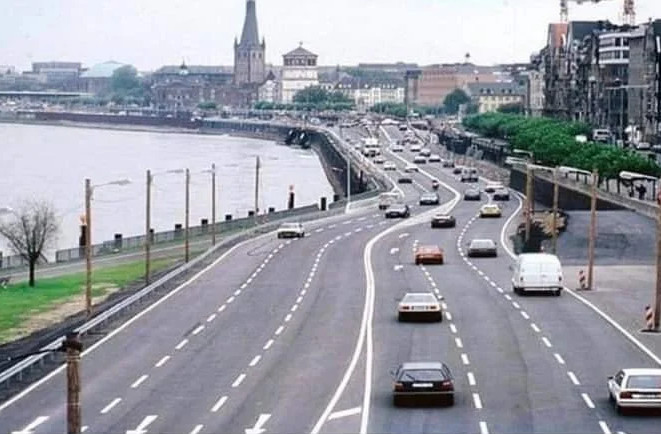
\includegraphics[scale=0.1, width=\textwidth]{images/dusseldorf1.jpg}<1->
	\only<2->{\begin{scriptsize}Düsseldorf, Germany (2019)\end{scriptsize}}
	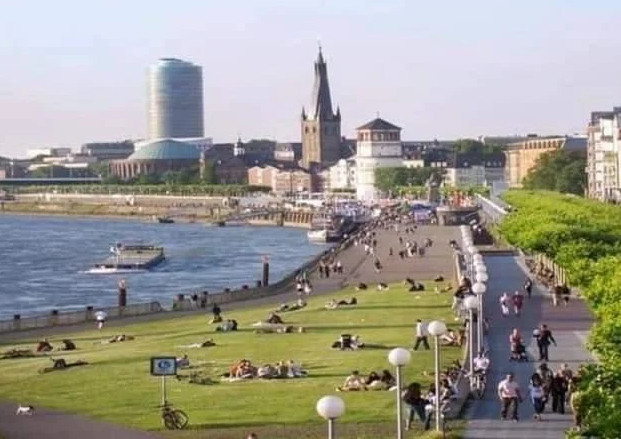
\includegraphics[scale=0.1, width=\textwidth]{images/dusseldorf2.jpg}<2->
\centering
\end{column}
\end{columns}
\end{frame}


\subsection{Use cases of the research}


\begin{frame}{Practical uses of the research}
\begin{columns}

\begin{column}{0.75\textwidth}
\begin{itemize}
	\item<1-> \textbf{Within-city}: Optimizing an existing piece of infrastructure
	\begin{itemize}
		\item Keep buildings intact
		\item Find optimal junction types
		\item Fine-tune lane capacities
	\end{itemize}
	\item<2-> \textbf{Green-field investment}: Only the junction locations are given. Everything else has to be found by the agent
	\begin{itemize}
		\item Lanes can be built freely between any two junctions
		\item Junction types can be set freely
	\end{itemize}
	\item<3-> \textbf{Mixed (reparation mode)}: Optimize an existing piece of infrastructure freely
	\begin{itemize}
		\item Lanes can be built between any two junctions
		\item Junction types can be set freely
	\end{itemize}
\end{itemize}
\end{column}

\begin{column}{0.3\textwidth}
	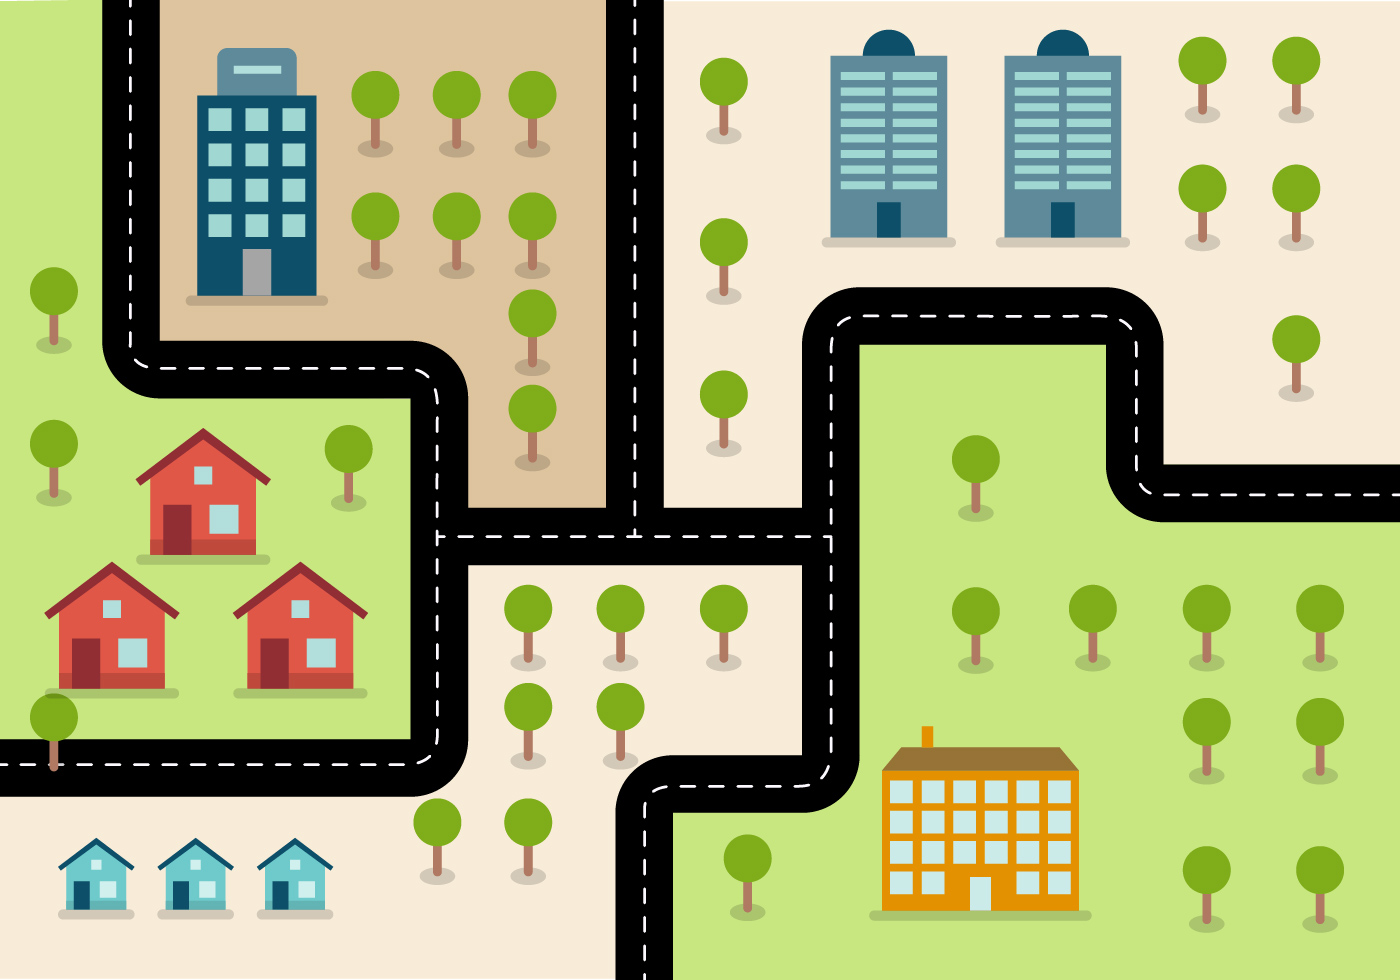
\includegraphics[scale=0.1, width=4cm, height=4cm]{images/within-city.jpg}<1>
	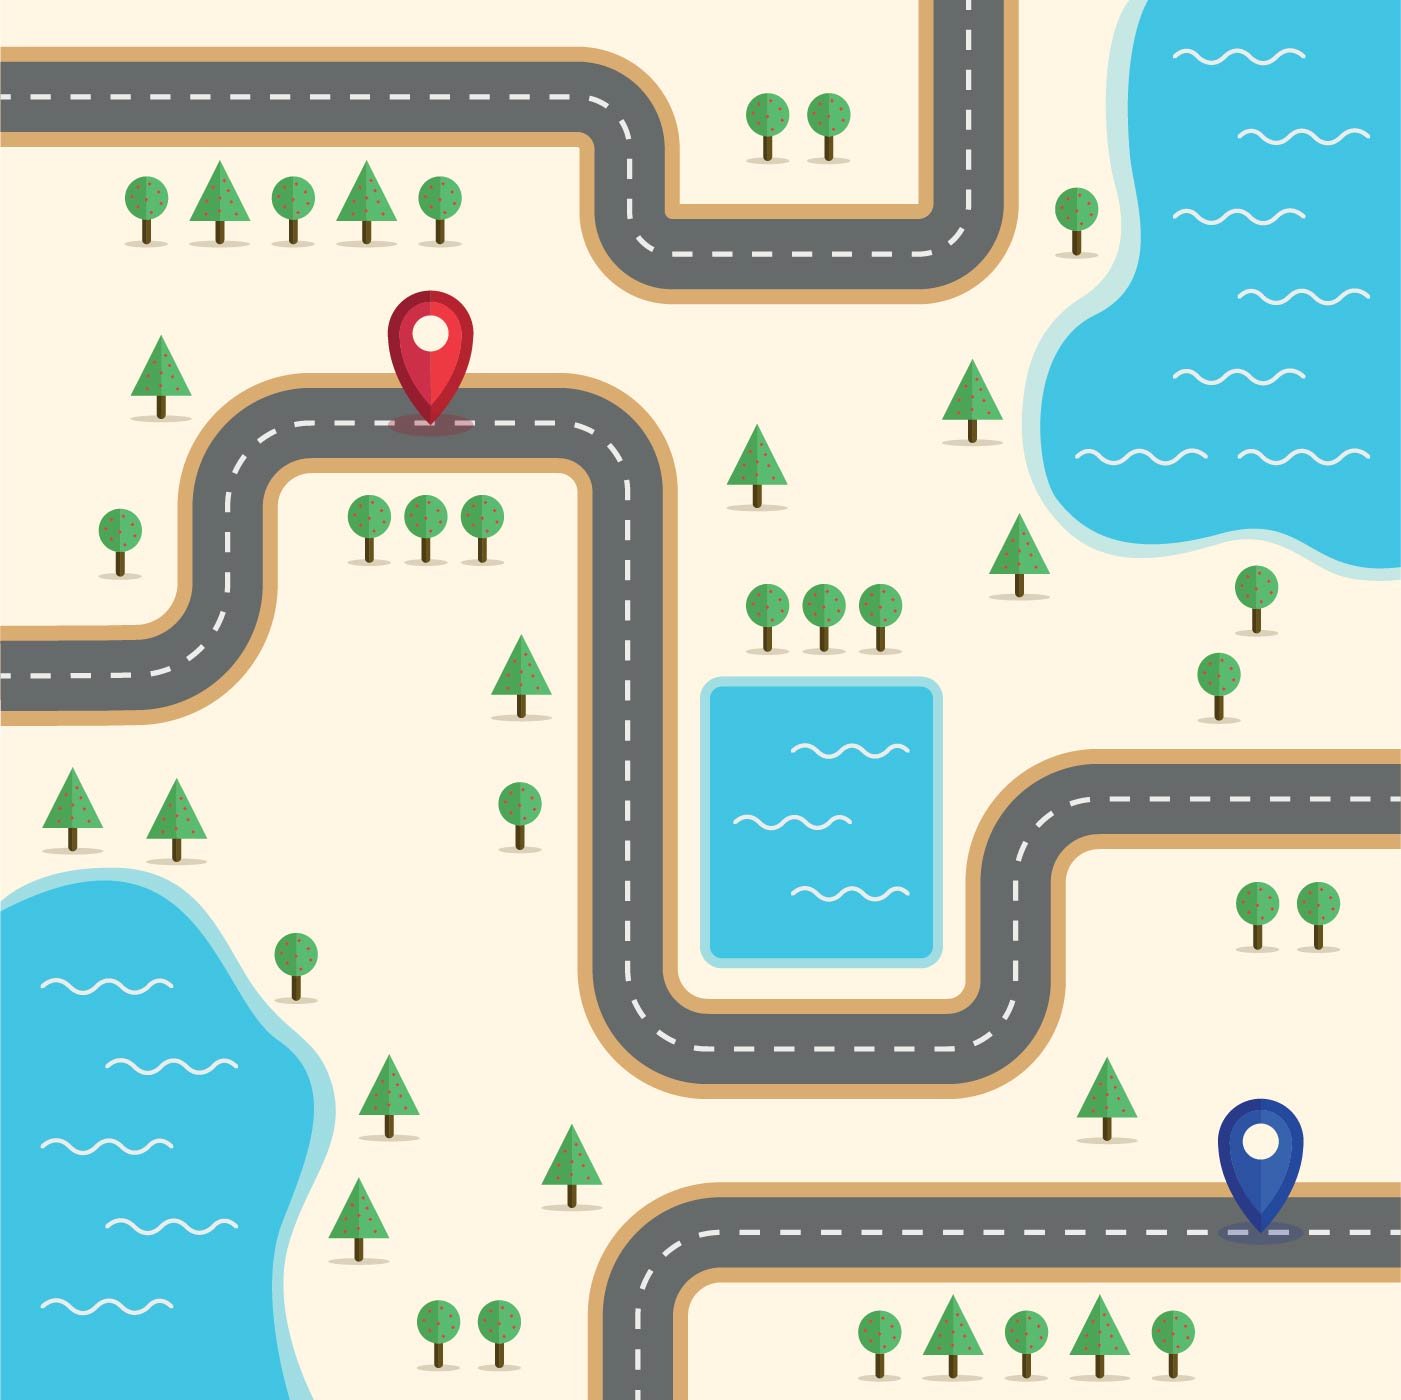
\includegraphics[scale=0.1, width=4cm, height=4cm]{images/green-field.jpg}<2>
	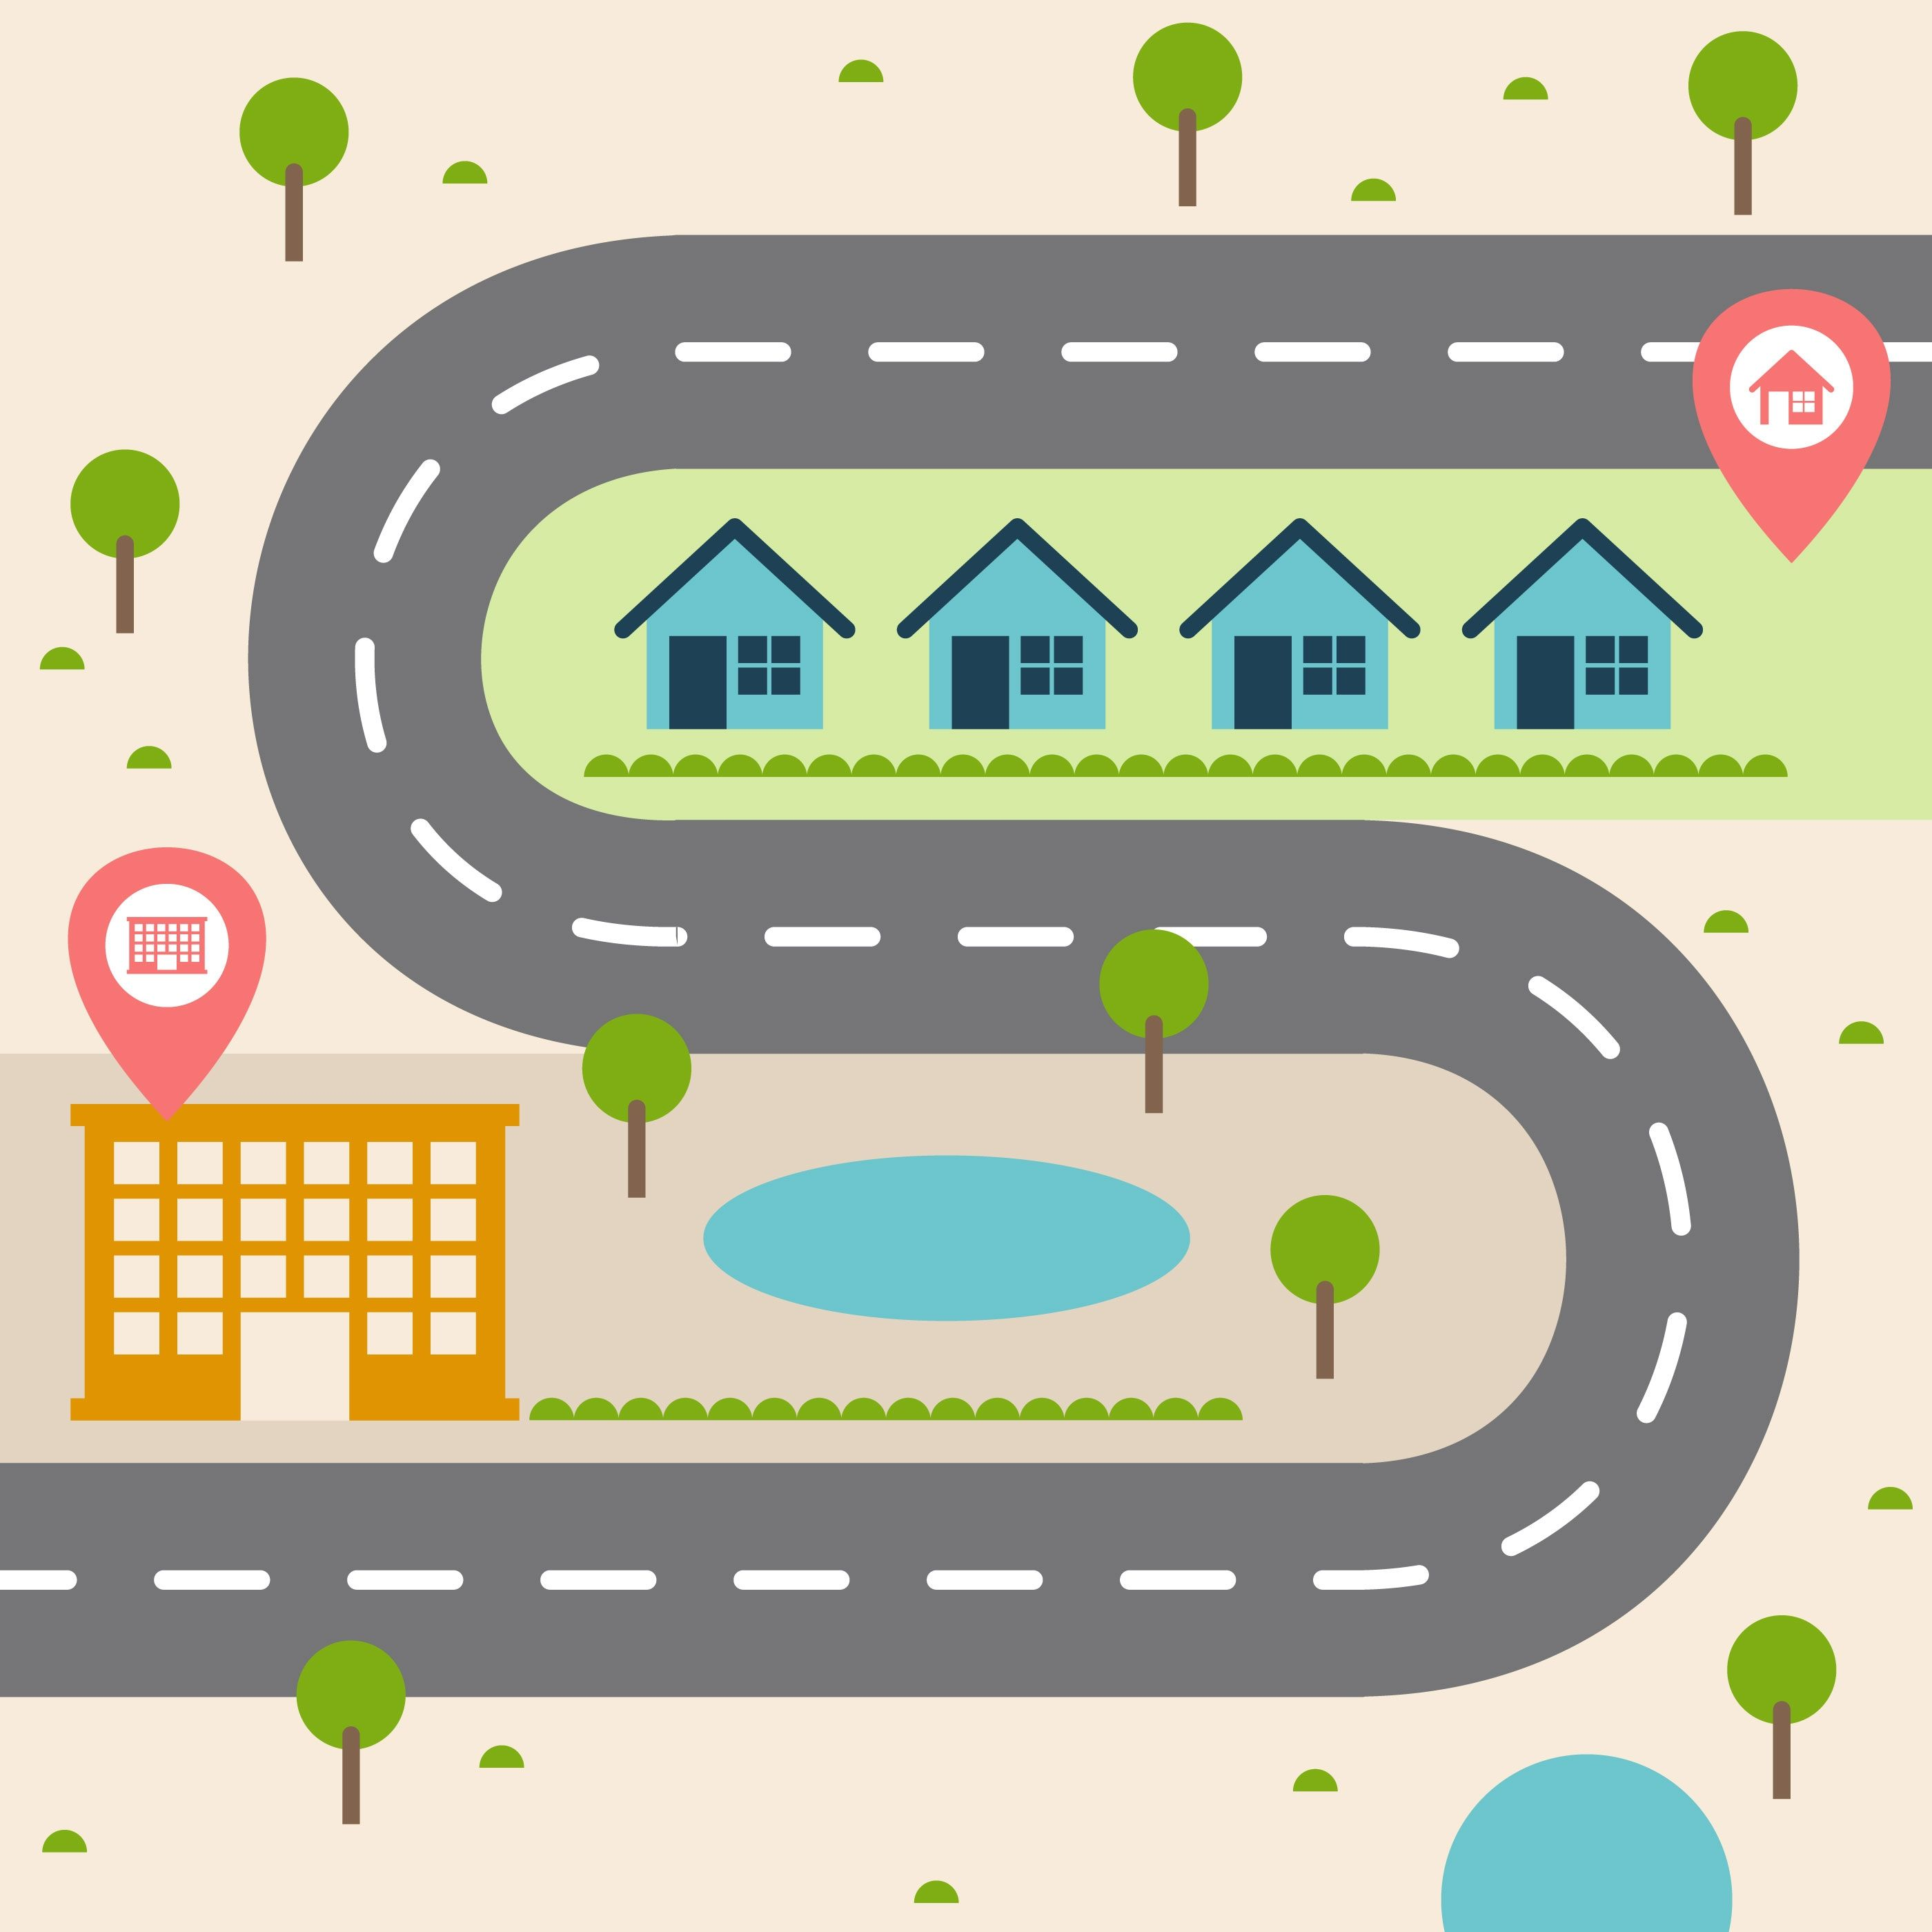
\includegraphics[scale=0.1, width=4cm, height=4cm]{images/mixed.jpg}<3>
\end{column}

\end{columns}
\end{frame}


\section{Methodology}

\begin{frame}
	\tableofcontents[currentsection]
\end{frame}

\subsection{Interface}


\begin{frame}{Constructing a city}
	A city is read into the program using a construction protocol. 
	The protocol stores the junctions and their relationships.
	\begin{center}

		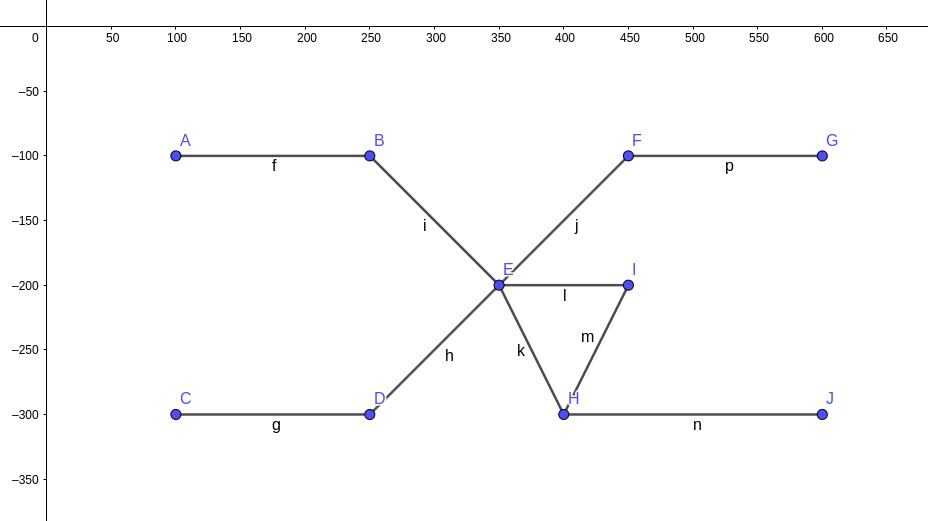
\includegraphics[height=5cm, keepaspectratio]{images/simple_graph.png}<1>
		\par % New paragraph		
		\only<1>{\begin{scriptsize}The design interface running in GeoGebra\end{scriptsize}}

		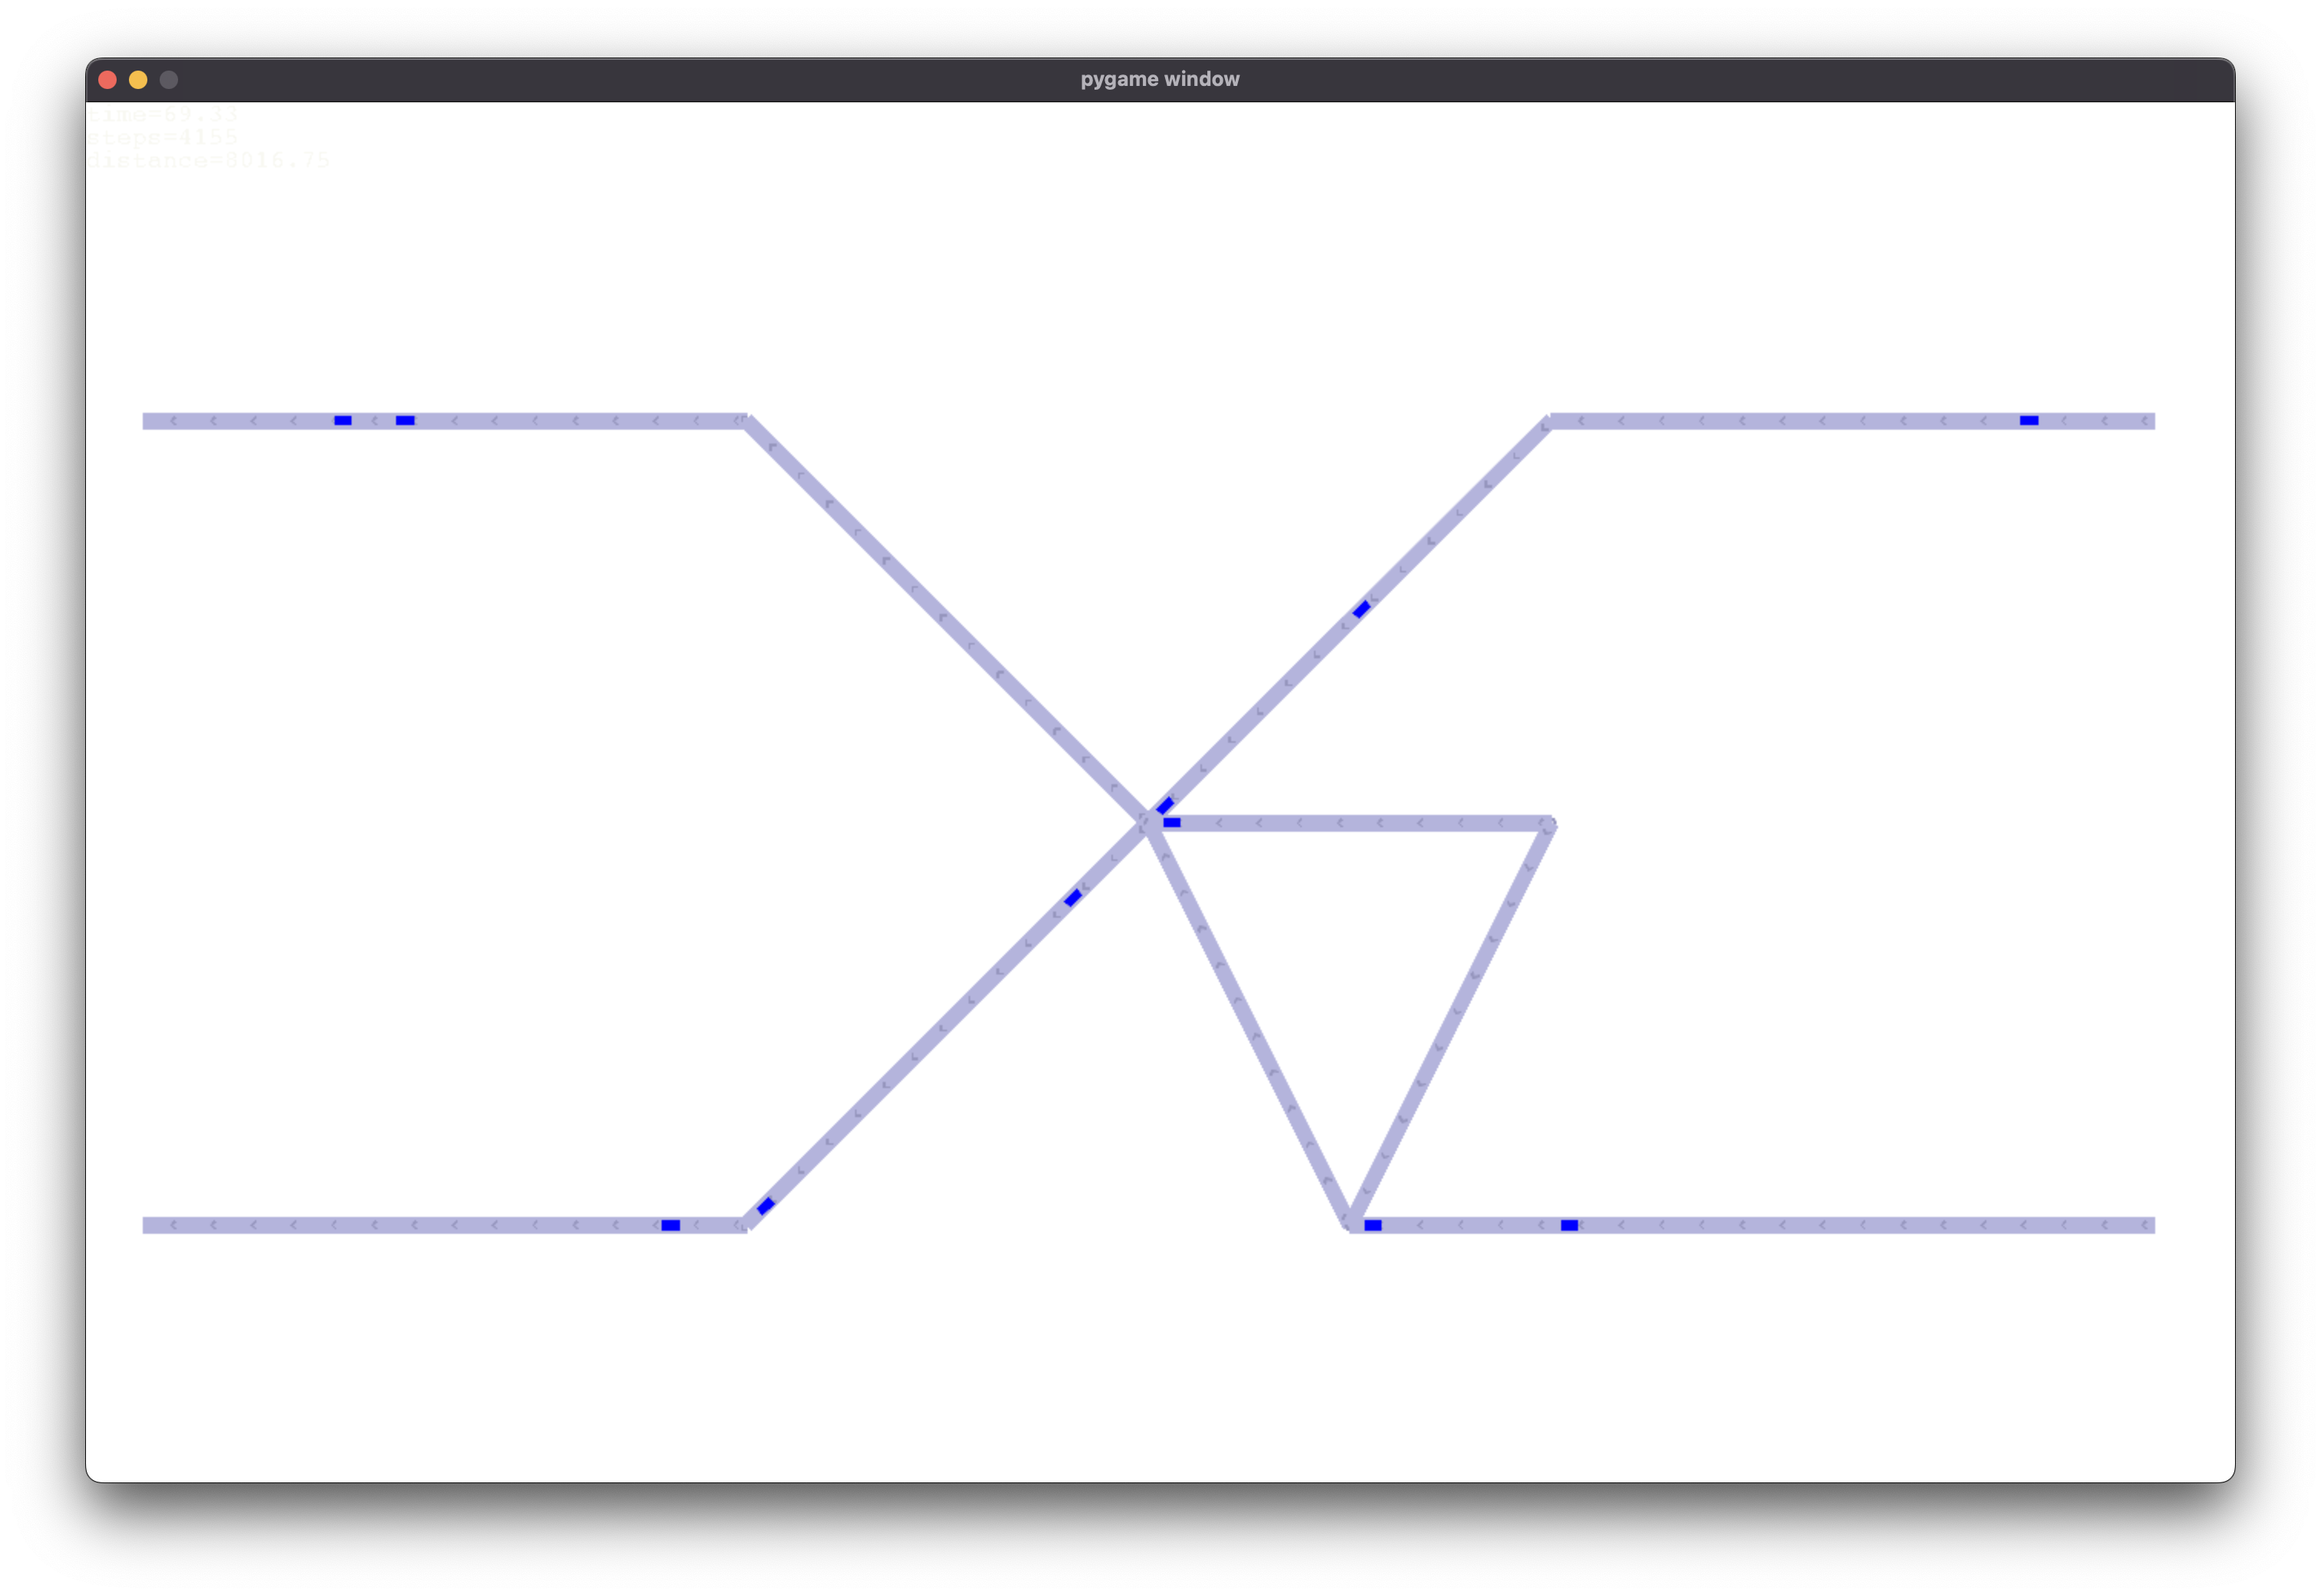
\includegraphics[height=5cm, keepaspectratio]{images/simple.png}<2>	
		\par
		\only<2>{\begin{scriptsize}The same city loaded into the simulation\end{scriptsize}}

	\end{center}
\end{frame}


\subsection{Simulation}


\begin{frame}{Running the simulation}
\begin{columns}

\begin{column}{0.4\textwidth}
	The drivers behave according to the intelligent driver model. The model defines:
	\begin{itemize}
		\item Maximum speed: $v_{0}$
		\item Safe following distance: $T$
		\item Maximum acceleration: $a$
		\item Comfortable deceleration: $b$
		\item Acceleration exponent: $\delta$
		\item Comfortable following distance: $s_{0}$
	\end{itemize}
\end{column}

\begin{column}{0.6\textwidth}
	\begin{block}{Intelligent driver model for vehicle $\alpha$}	
		\begin{scriptsize}
		\begin{equation*}
		\dot{v}_{\alpha}=a^{(\alpha)}\left[1-\left(\frac{v_{\alpha}}{v_{0}^{(\alpha)}}\right)^{\delta}-\left(\frac{s^{*}(v_{\alpha},\Delta v_{\alpha})}{s_{\alpha}}\right)^{2}\right]
		\end{equation*}
		
		\end{scriptsize}
	\end{block}	
	
	\begin{center}
	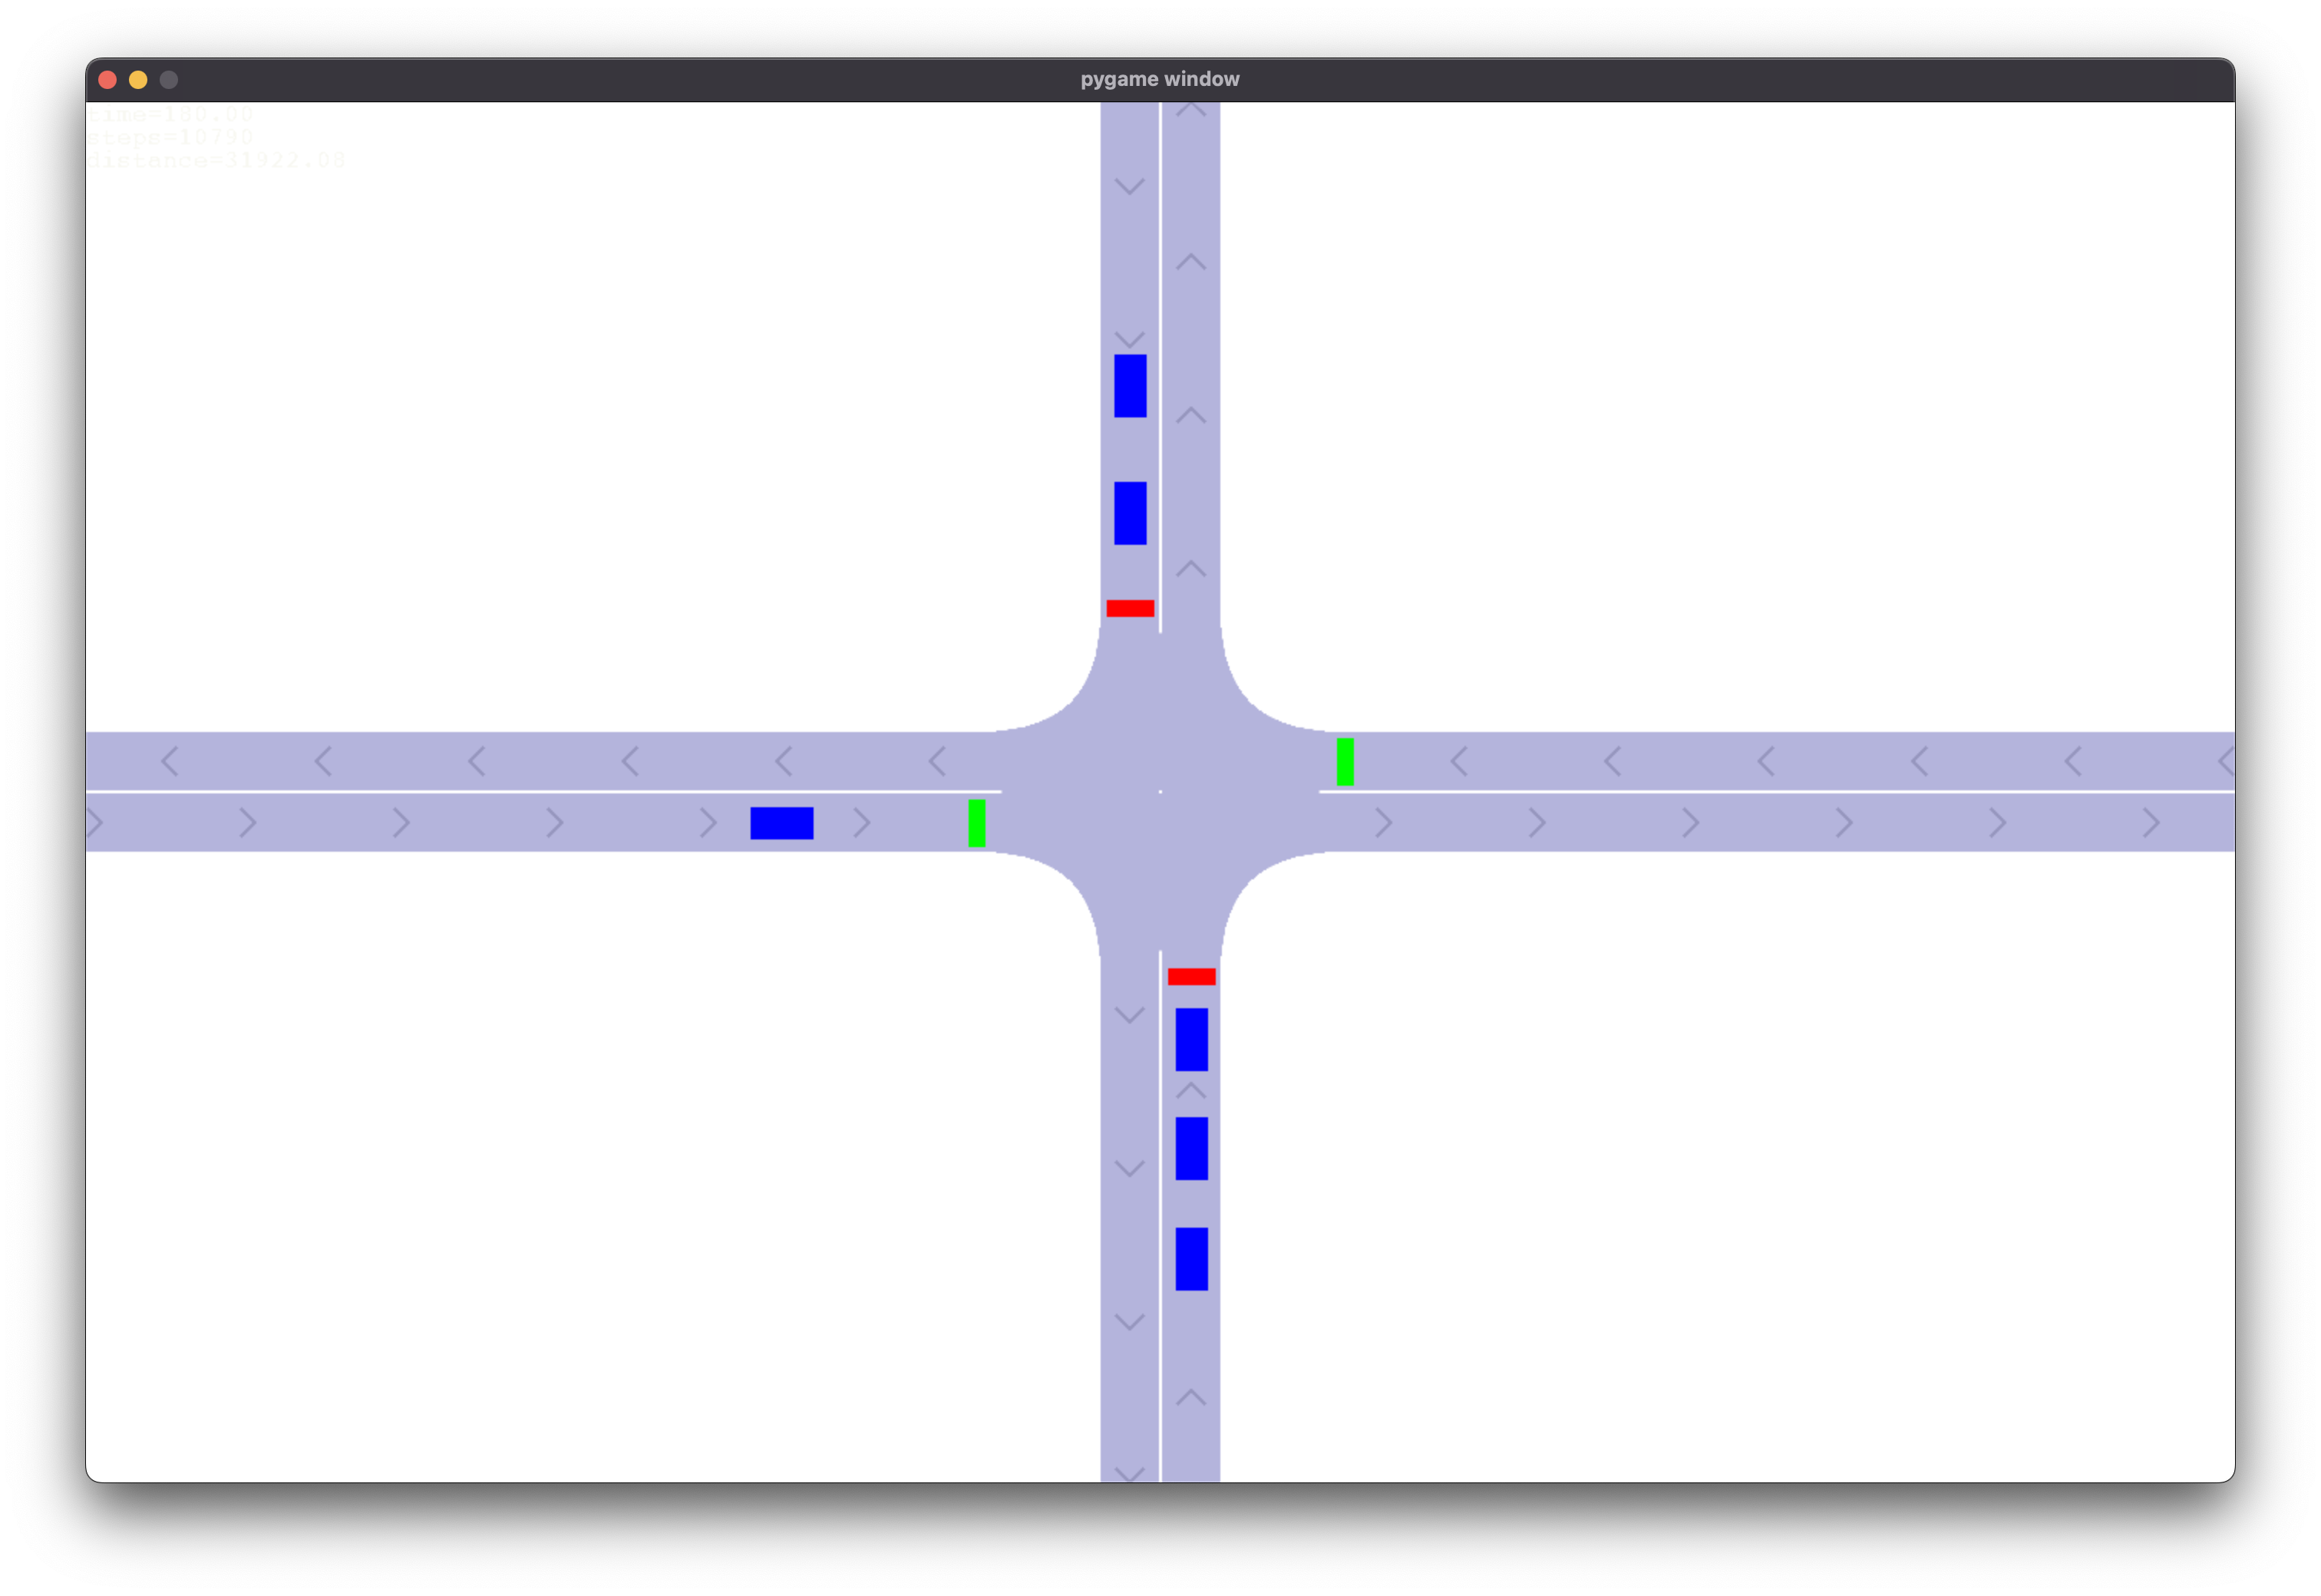
\includegraphics[width=5cm, keepaspectratio]{images/junction_trafficlight.png}
	\par	
	\begin{scriptsize}Vehicles in the simulation\end{scriptsize}
	\end{center}	
	
\end{column}
\end{columns}
\end{frame}


\subsection{Modeling}

\begin{frame}{The RL task}
\begin{columns}
\begin{column}{0.5\textwidth}
	The task of the agent is to predict the ending node and action from its current position. Each iteration the ending node will become the current position. The choice of actions are:
	\begin{itemize}
		\item Add a lane
		\item Remove a lane
		\item Build a right-hand intersection
		\item Build a roundabout
		\item Build a traffic light
	\end{itemize}
\end{column}

\begin{column}{0.5\textwidth}
	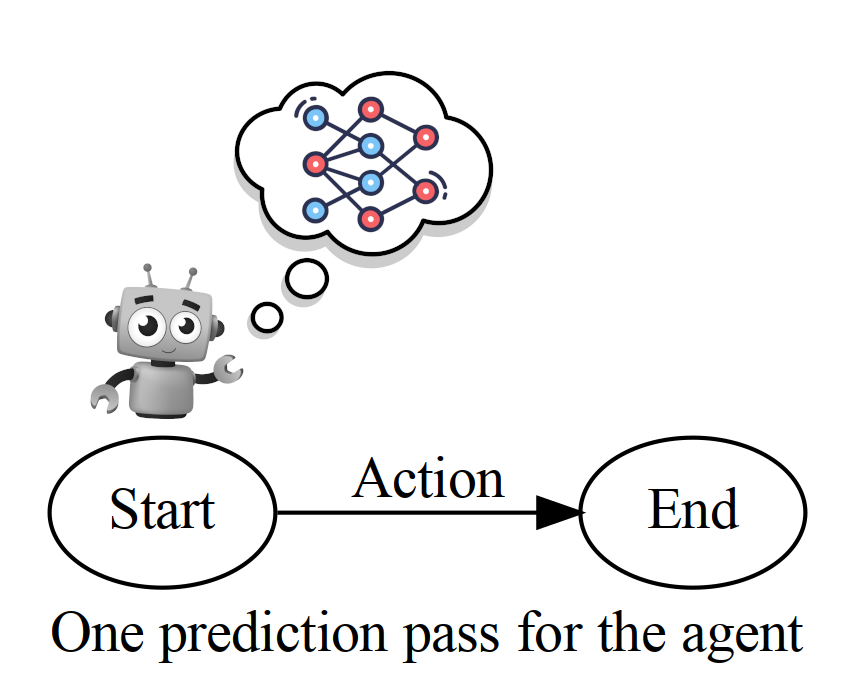
\includegraphics[scale=0.25]{images/rl_process.png}
\end{column}

\end{columns}
\end{frame}


\begin{frame}{State-based architecture}
\begin{columns}

\begin{column}{0.5\textwidth}<1->
	\begin{center}
	\begin{scriptsize}Ending node prediction architecture\end{scriptsize} 
	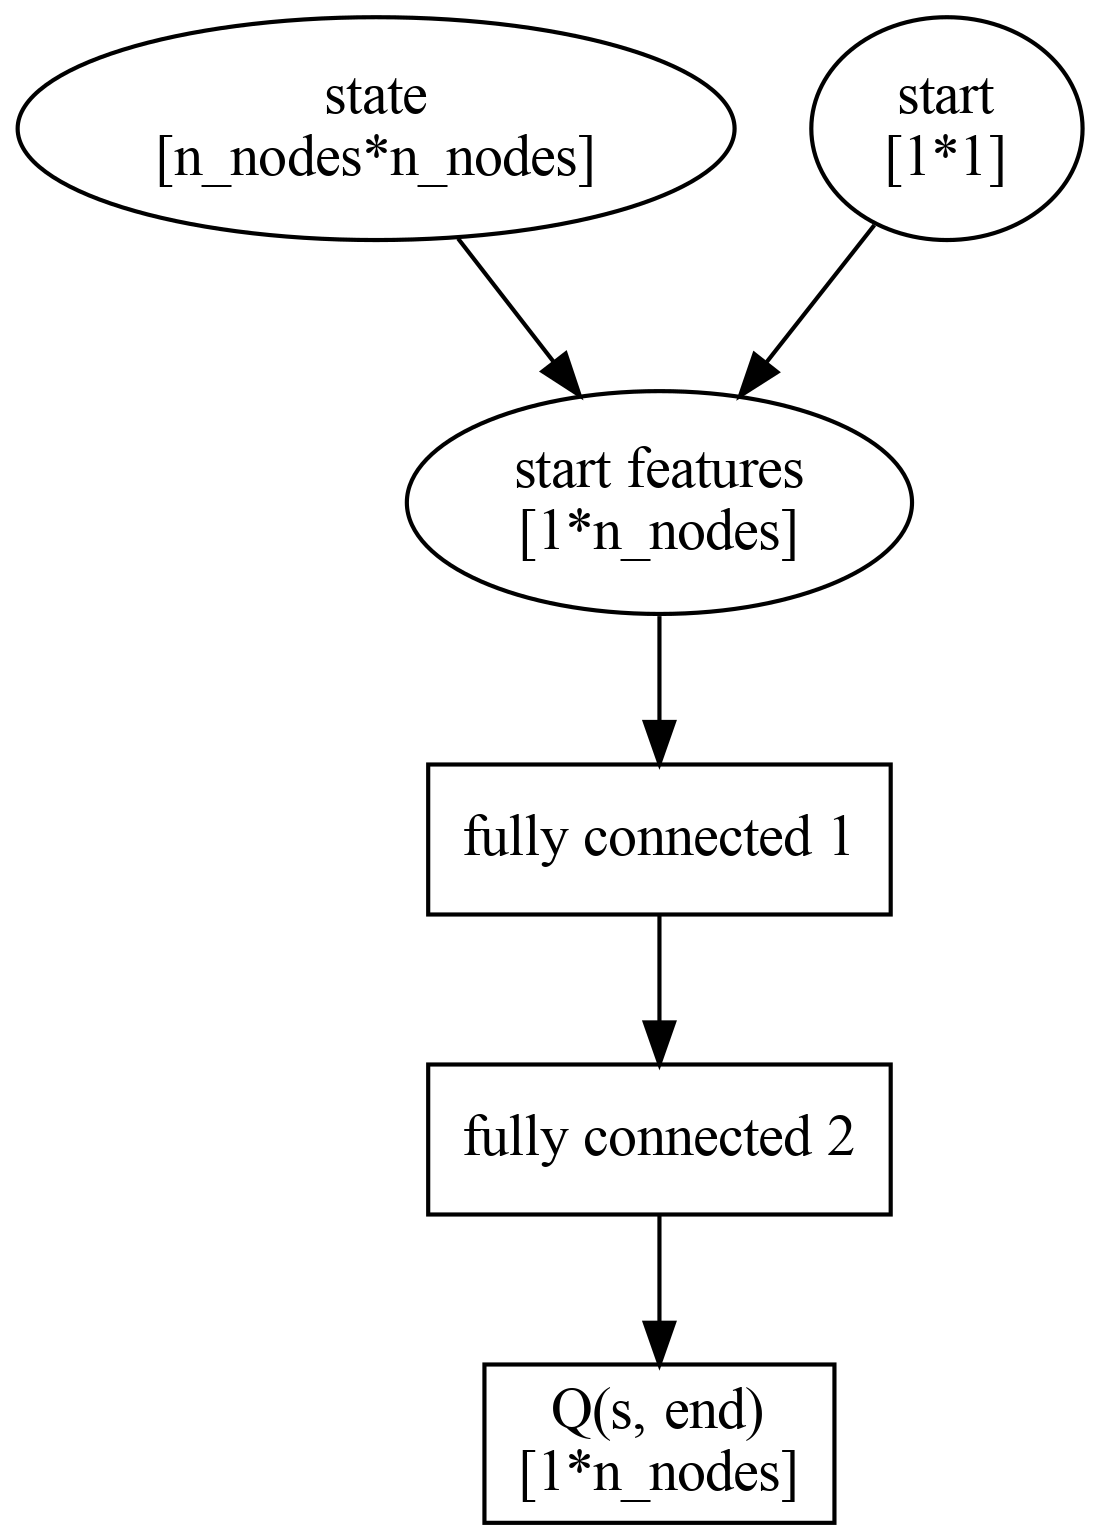
\includegraphics[height=6cm, keepaspectratio]{images/snn_end.png}	
	\end{center}
\end{column}

\begin{column}{0.5\textwidth}
	\begin{center}

	\only<1>{
		\begin{block}{The state of the system}
		\begin{scriptsize}
			The graph of the city is represented by its adjacency matrix. For $n$ nodes the descriptor matrix $x$ is of size $n*n$. The diagonal elements $x(N_{i},N_{i})$ describe the self-connections e.g. the type of intersection that can be found at junction $N_{i}$ in the city. All other connections $x(N_{i},N_{j}),\,i\neq j$ represent the number of lanes between nodes $N_{i},N_{j}$.		
		\end{scriptsize}
		\end{block}
	}	
	
	\only<2>{\begin{scriptsize}Action prediction architecture\end{scriptsize}}
	\only<2>{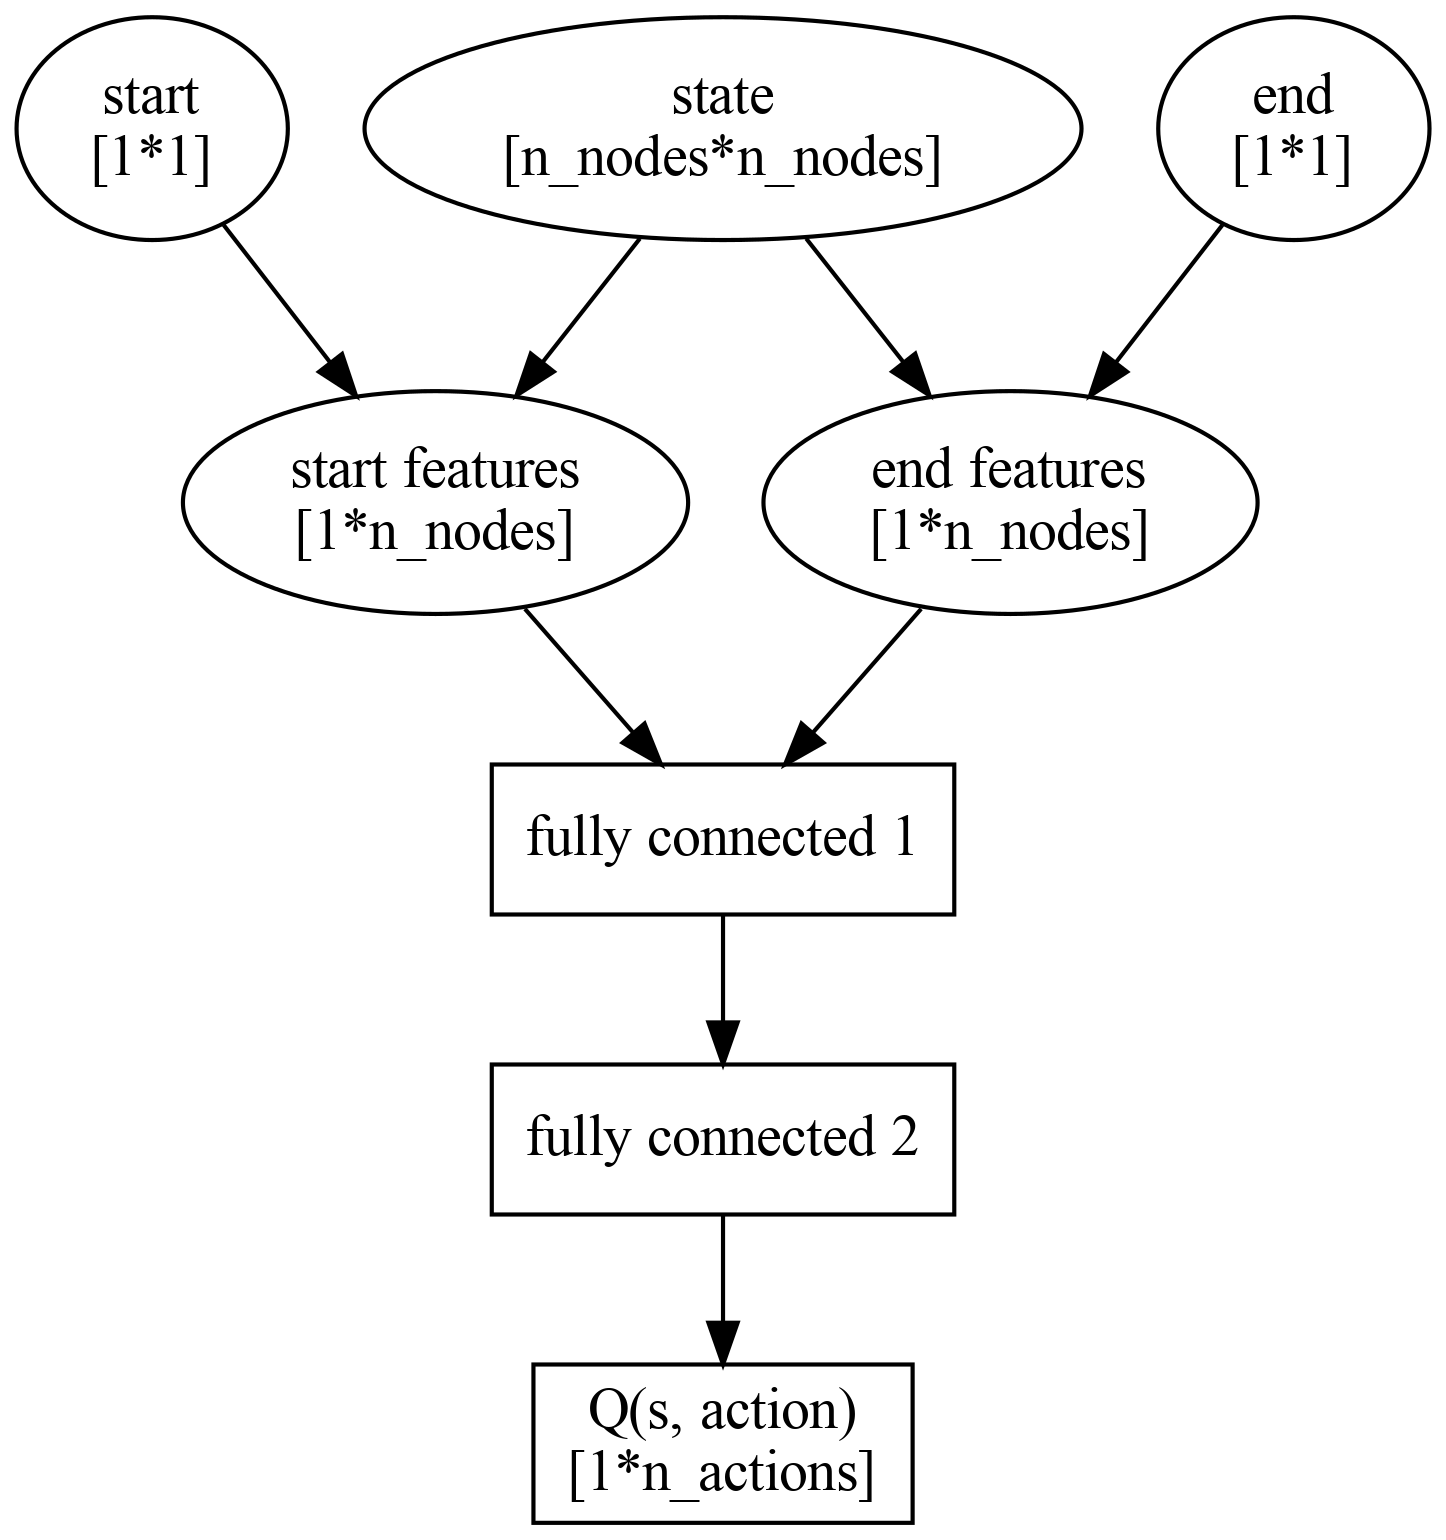
\includegraphics[height=6cm, keepaspectratio]{images/snn_action.png}}
	
	\end{center}
\end{column}

\end{columns}
\end{frame}


\begin{frame}{State-embedding-based architecture}
\begin{columns}

\begin{column}{0.5\textwidth}<1->
	\begin{center}
	\begin{scriptsize}Ending node prediction architecture\end{scriptsize} 
	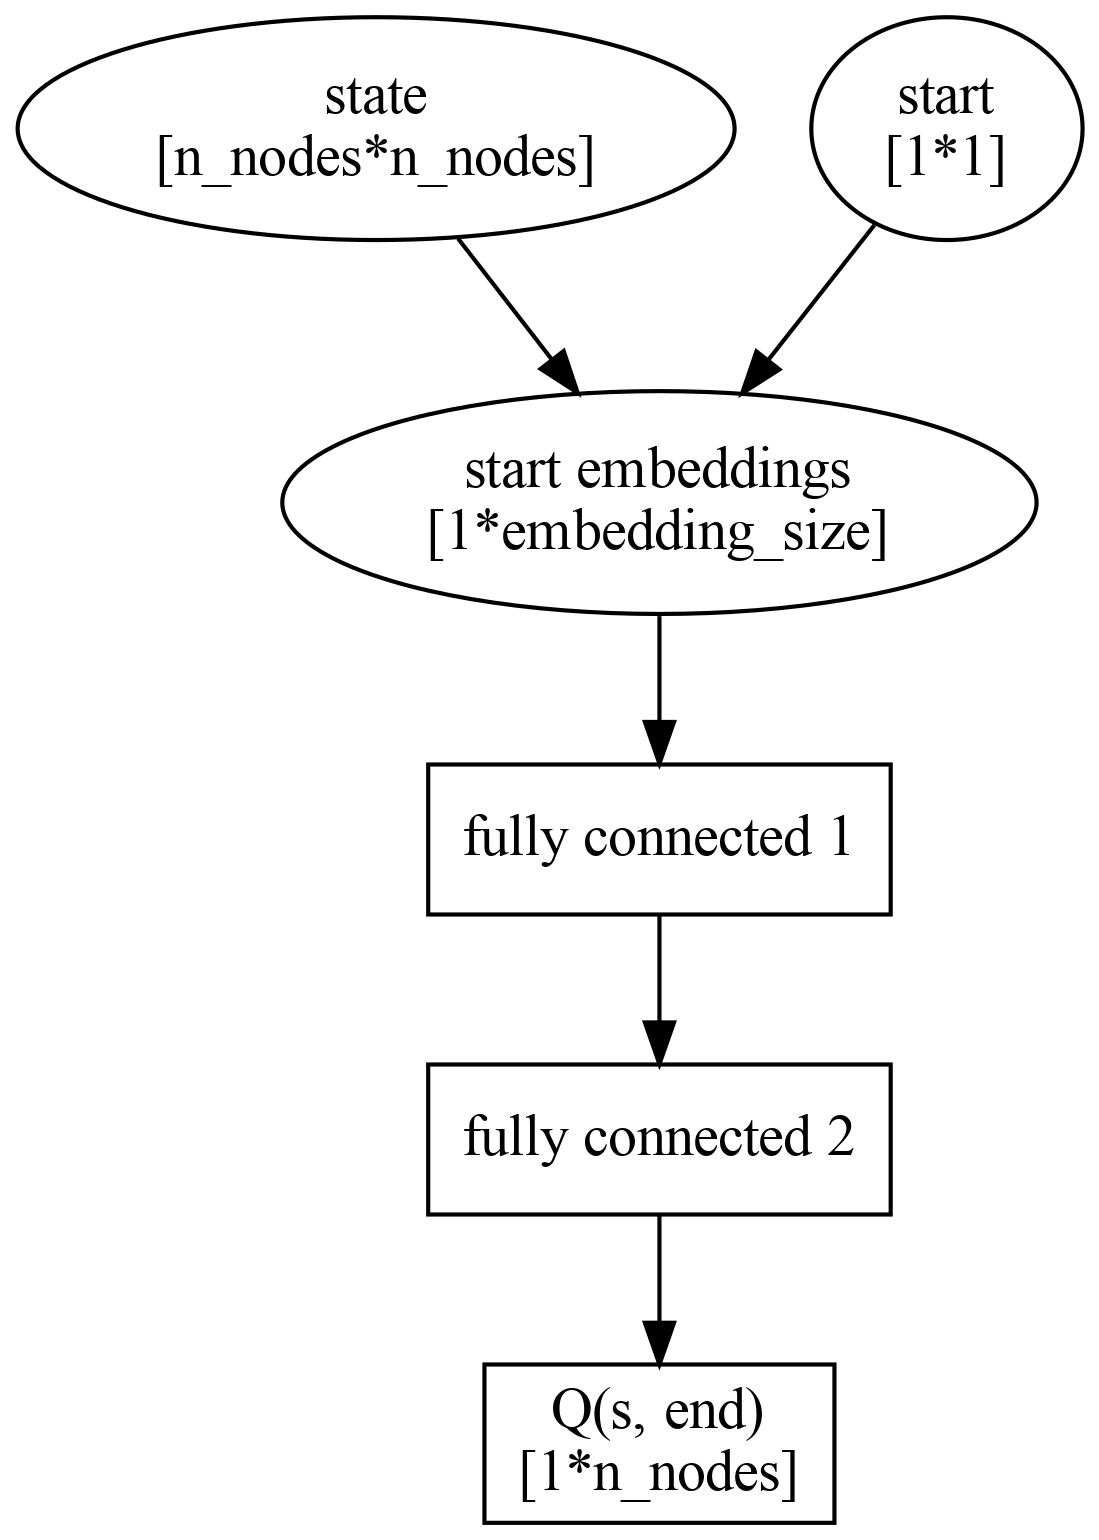
\includegraphics[height=6cm, keepaspectratio]{images/enn_end.png}	
	\end{center}
\end{column}

\begin{column}{0.5\textwidth}
	\begin{center}
	
	\only<1>{
	\begin{block}{Embeddings with graph-structured data}
	\begin{scriptsize}
	In graph neural networks (GNN) embeddings are used to capture the structure and relationships within the graph, allowing the network to perform tasks such as link prediction and node classification.
	\end{scriptsize}
	\end{block}
	}	
	
	\only<2>{\begin{scriptsize}Action prediction architecture\end{scriptsize}}
	\only<2>{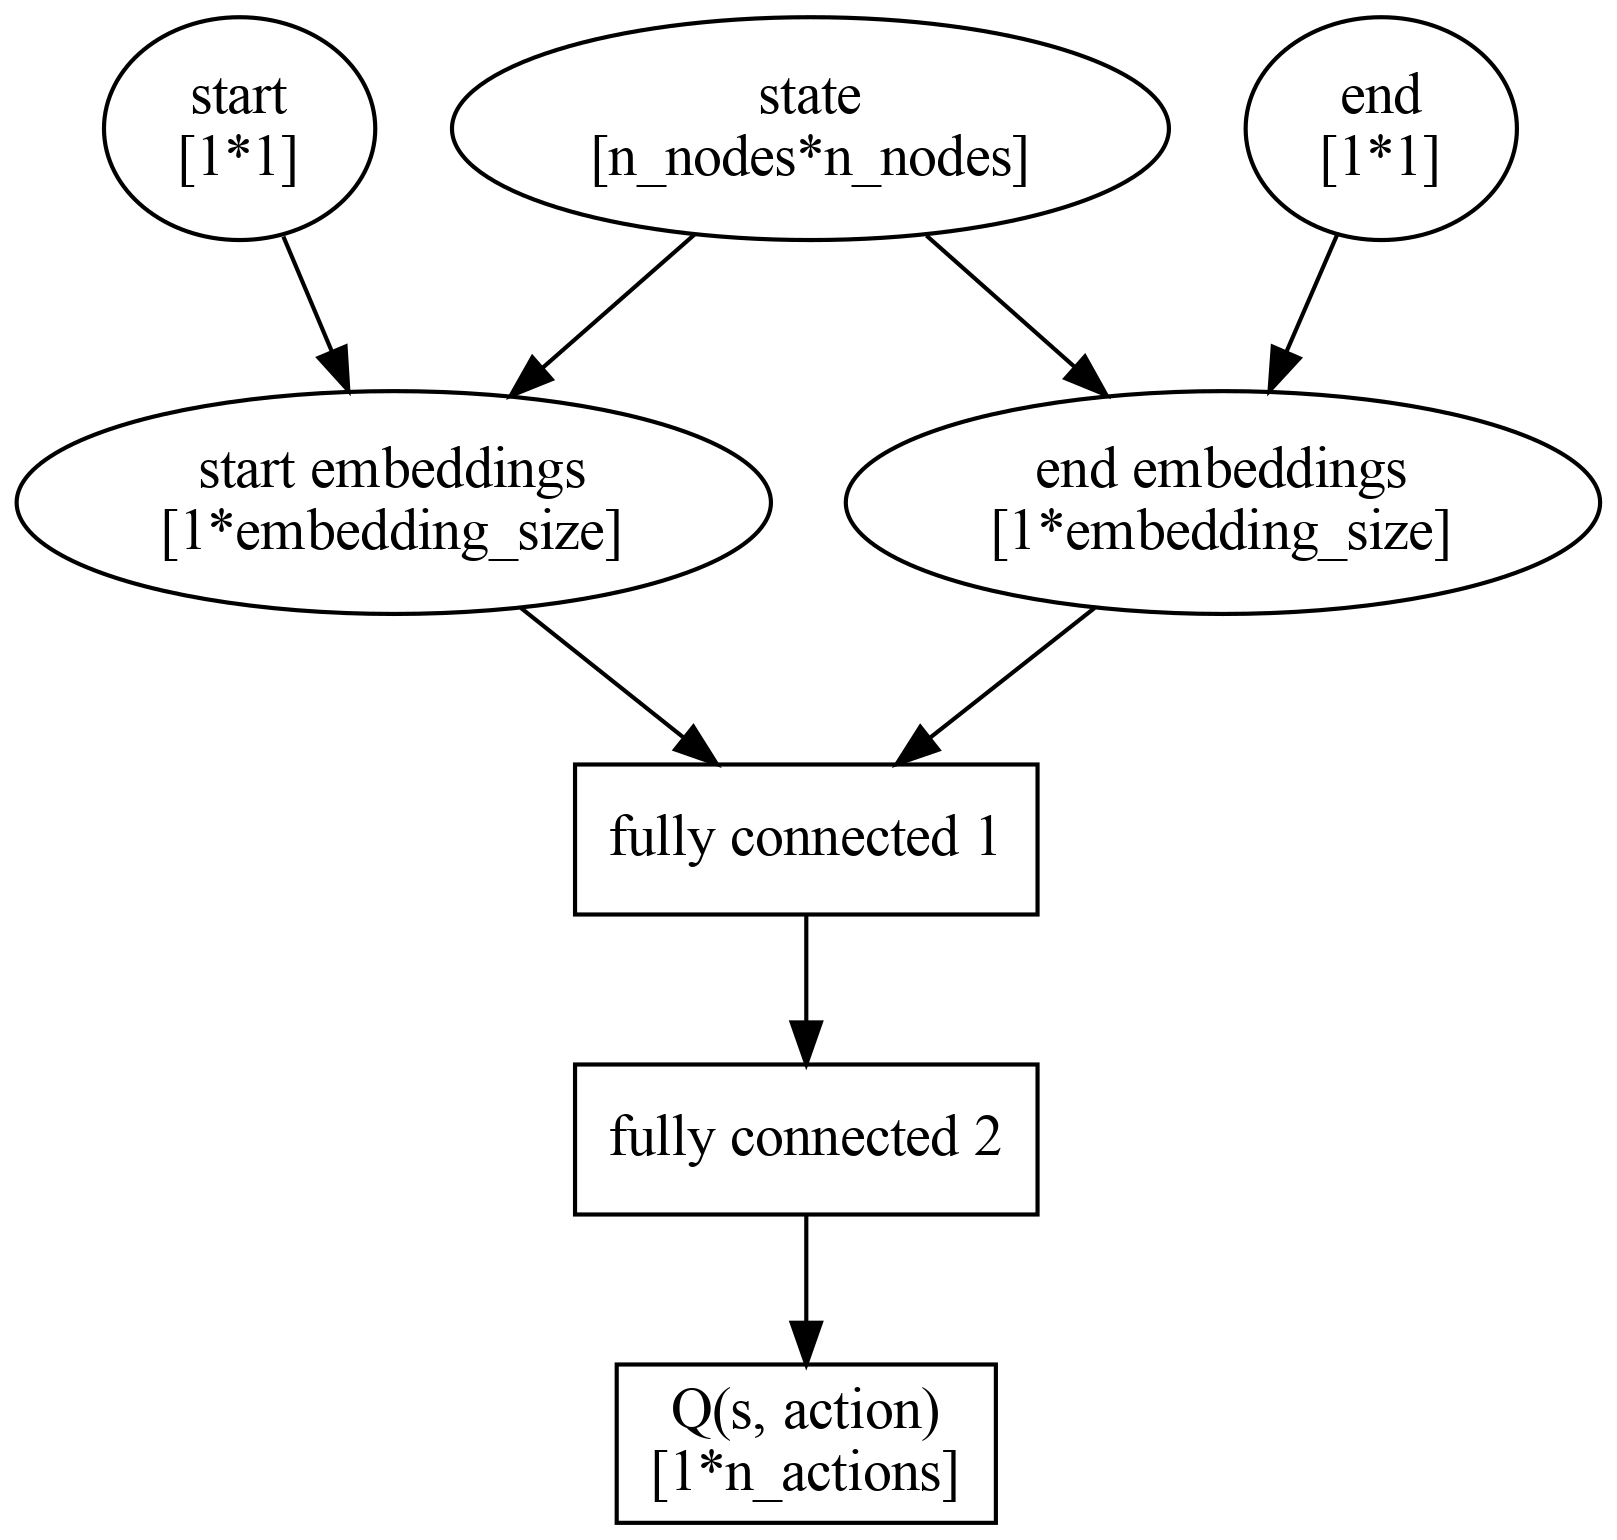
\includegraphics[height=6cm, keepaspectratio]{images/enn_action.png}}
	\end{center}
\end{column}

\end{columns}
\end{frame}


\begin{frame}{Graph-convolutional architecture}
\begin{columns}

\begin{column}{0.4\textwidth}<1->
	\begin{center}
	\begin{scriptsize}Ending node prediction architecture\end{scriptsize} 
	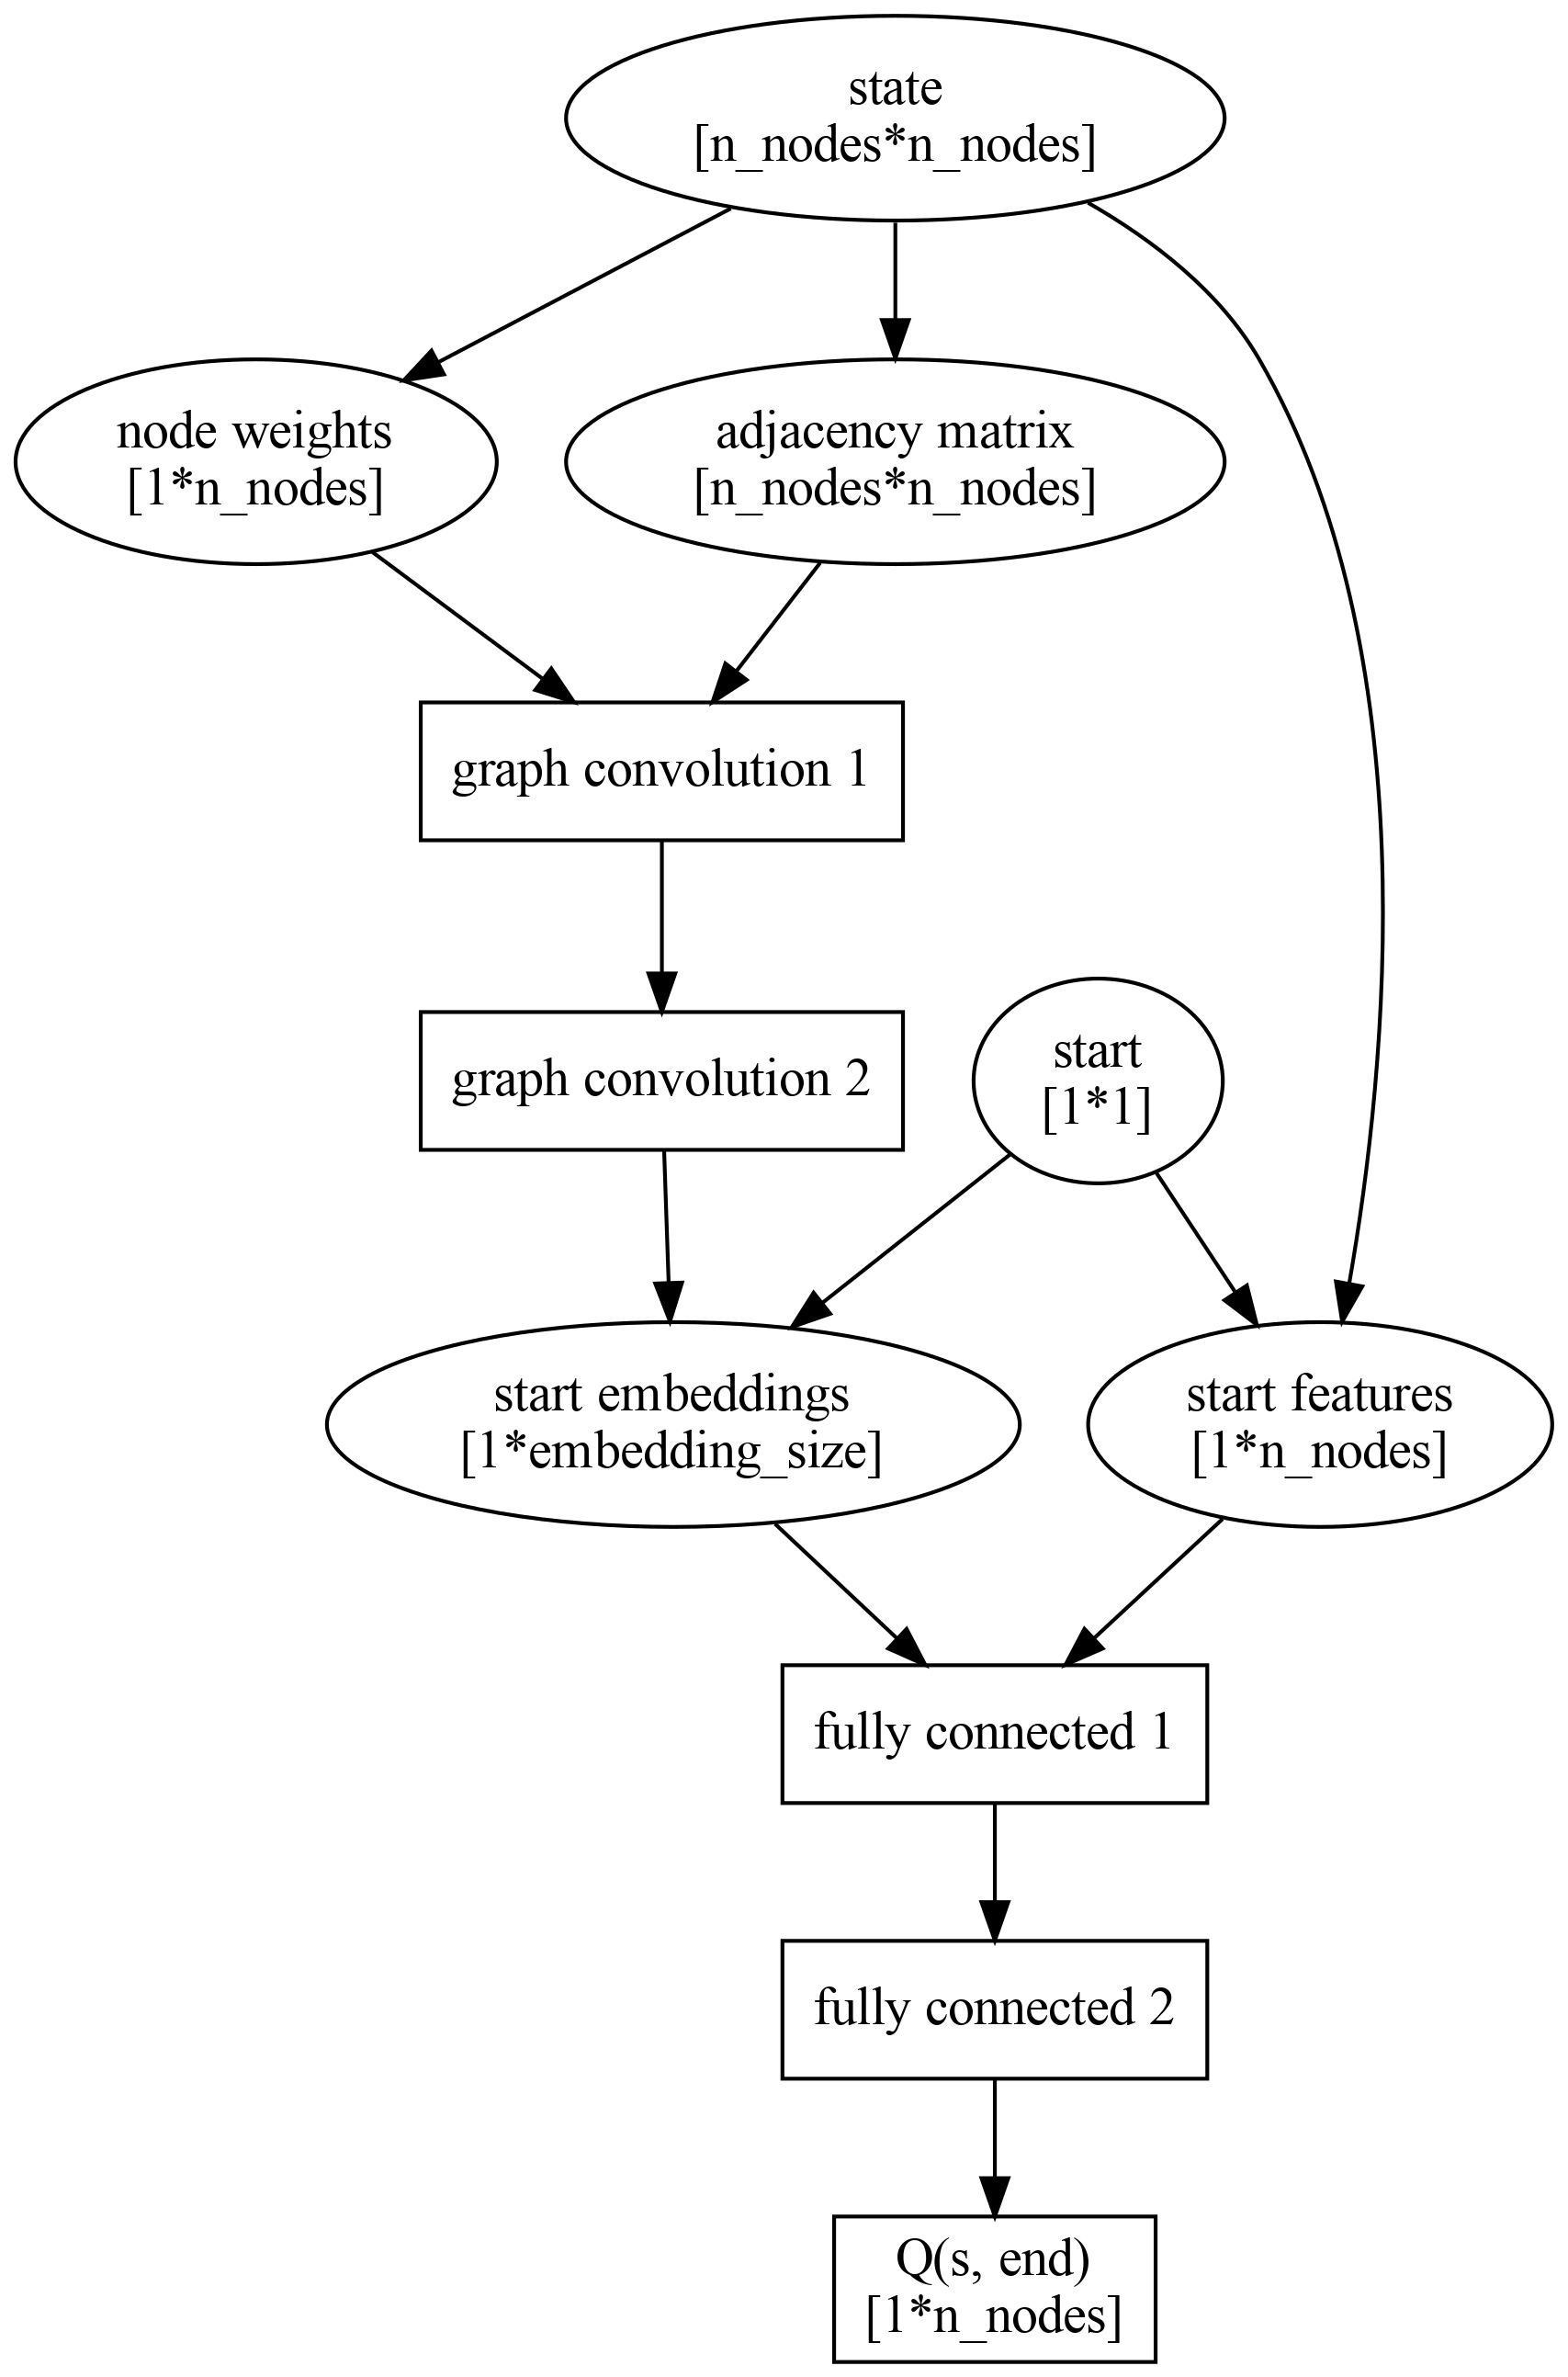
\includegraphics[height=6cm, keepaspectratio]{images/gcnn_end.png}	
	\end{center}
\end{column}

\begin{column}{0.6\textwidth}
	\begin{center}	

	
	\only<1>{
		\begin{block}{The propagation rule for GCN}
		\begin{equation*}
		H^{(l+1)}=\sigma\left(\tilde{D}^{-\frac{1}{2}}\tilde{A}\tilde{D}^{-\frac{1}{2}}H^{(l)}W^{(l)}\right)
		\end{equation*}
		
		\begin{flushleft}
		\begin{itemize}
		\begin{scriptsize}
			\item $\sigma(.)$ is the activation function
			\item $\tilde{D_{ii}}=\sum_{j}\tilde{A}_{ij}$ is the degree matrix of the graph
			\item $\tilde{A}=A+I_{N}$ is the graph's adjacency matrix including self-connections
			\item $W^{(l)}$ are the trainable weights of the layers
			\item $H^{(l)}$ denotes the activations of the $l$-th layer of the network
		\end{scriptsize}
		\end{itemize}
		\end{flushleft}		
		
		\end{block}
	}
	
	\only<2>{\begin{scriptsize}Action prediction architecture\end{scriptsize}}
	\only<2>{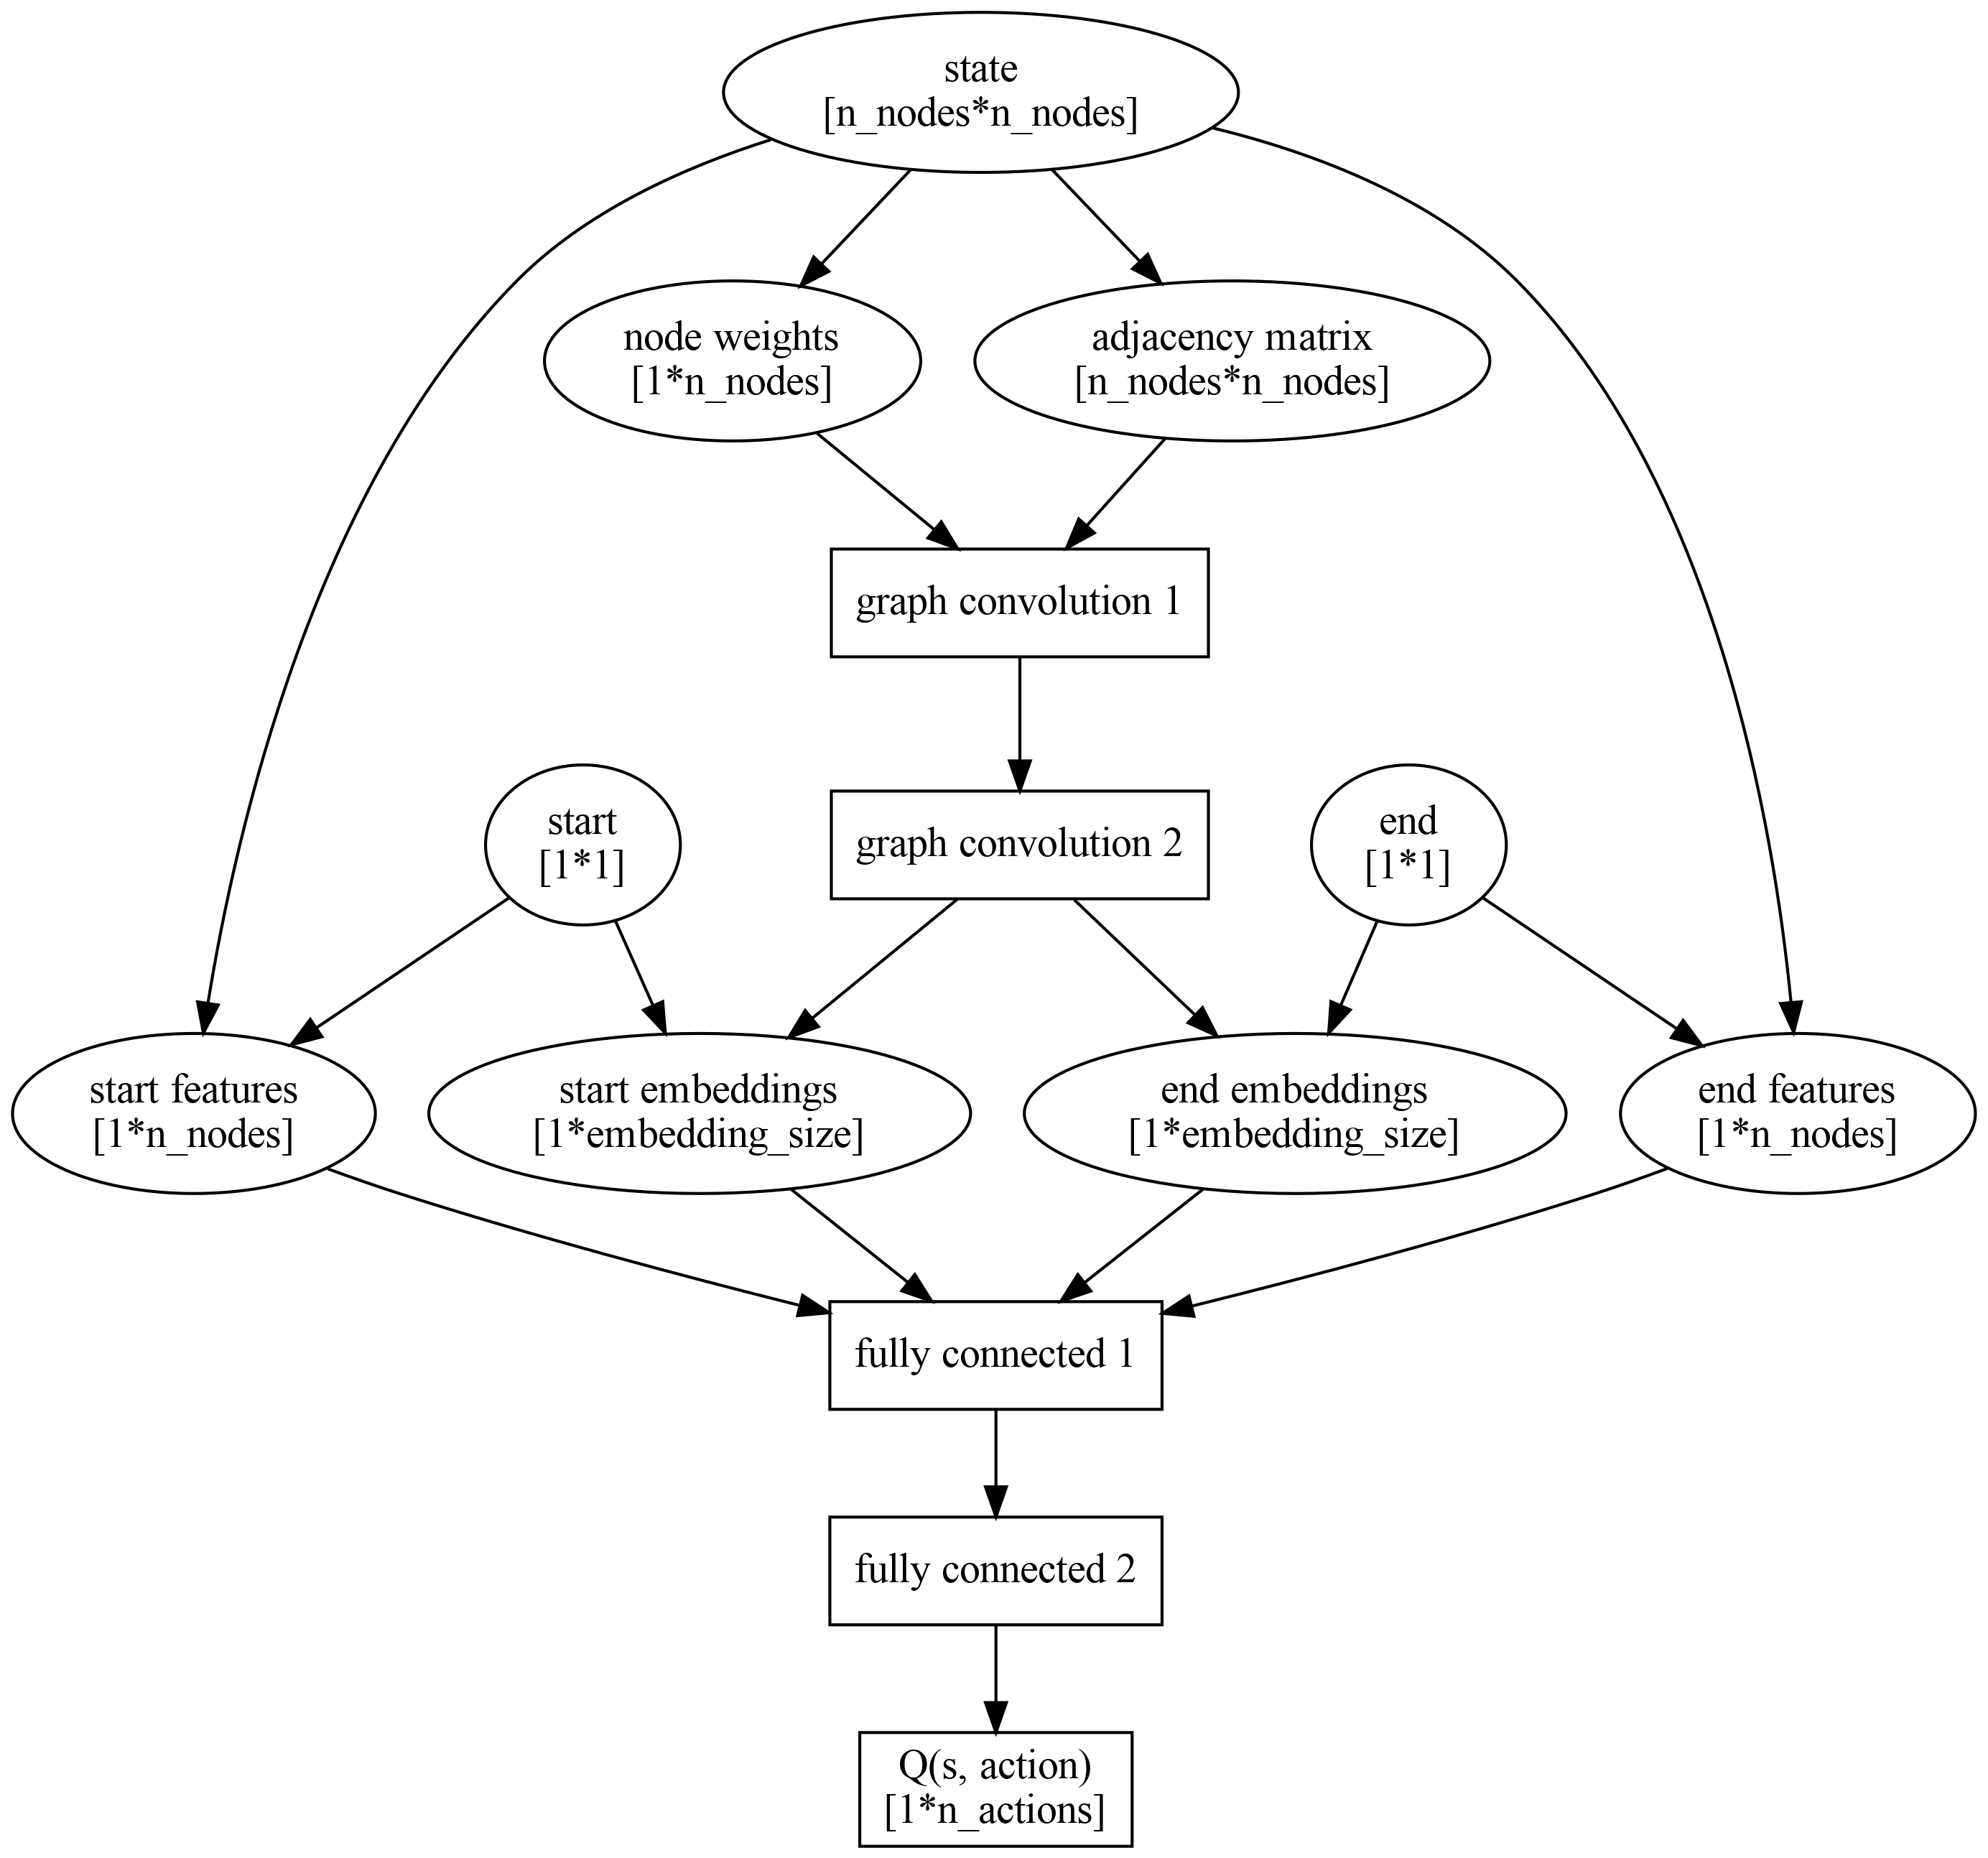
\includegraphics[height=6cm, keepaspectratio]{images/gcnn_action.png}}
	\end{center}
\end{column}

\end{columns}
\end{frame}


\subsection{Testing environment}

\begin{frame}{Testing environment}
\begin{columns}

\begin{column}{0.5\textwidth}
	\begin{center}
	The mixed configuration
	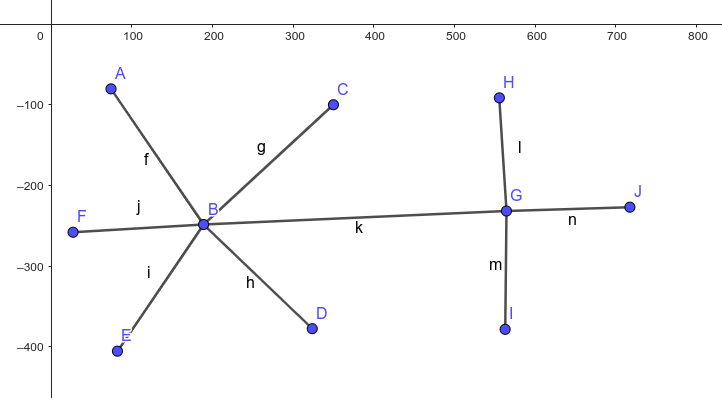
\includegraphics[width=6cm, keepaspectratio]{images/test_5_intersection.png}
	\end{center}
	\begin{itemize}
		\item The two intersections are bottlenecks
		\item All junctions are right-hand by default
		\item The roads have one lane in each direction
	\end{itemize}
\end{column}

\begin{column}{0.5\textwidth}
	\begin{center}
	The green-field configuration
	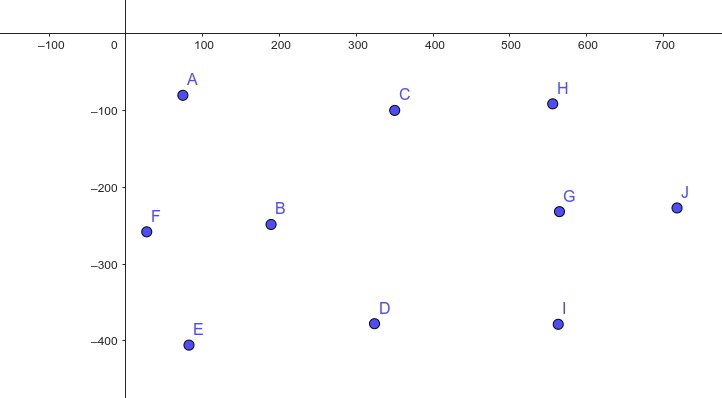
\includegraphics[width=6cm, keepaspectratio]{images/test_5_intersection_empty.png}
	\end{center}
	\begin{itemize}
		\item Only the locations of the junctions are given
		\item The agent has to build everything from scratch
	\end{itemize}
\end{column}

\end{columns}
\end{frame}


\section{Results}

\begin{frame}
	\tableofcontents[currentsection]
\end{frame}

\subsection{Episodic rewards}


\begin{frame}{Episodic rewards for training}
\begin{columns}

\begin{column}{0.65\textwidth}
	\begin{itemize}
		\item The training was ran for 1000 episodes
		\item The performance was measured for all 3 models
		\item The unit of measurement is the cumulated reward over 15 building steps
		\item A city design at time step $t$ is scored using the formula:		
		
		\begin{scriptsize}		
		\begin{align*}
			score_{city}^{t}=-cost_{infrastructure}^{t}+score_{human}^{t}+score_{vehicular}^{t}
		\end{align*}	
		\end{scriptsize}		
			
		\item The reward signal is calculated as the difference in city scores:
		
		\begin{scriptsize}
		\begin{align*}		
			r_{t}=\delta_{score_{city}}=-(score_{city}^{t-1}-score_{city}^{t})
		\end{align*}				
		\end{scriptsize}

	\end{itemize}
\end{column}

\begin{column}{0.5\textwidth}
	\begin{center}

	\begin{scriptsize}
	
	\only<1>{Unsmoothed rewards (mixed mode)}	
	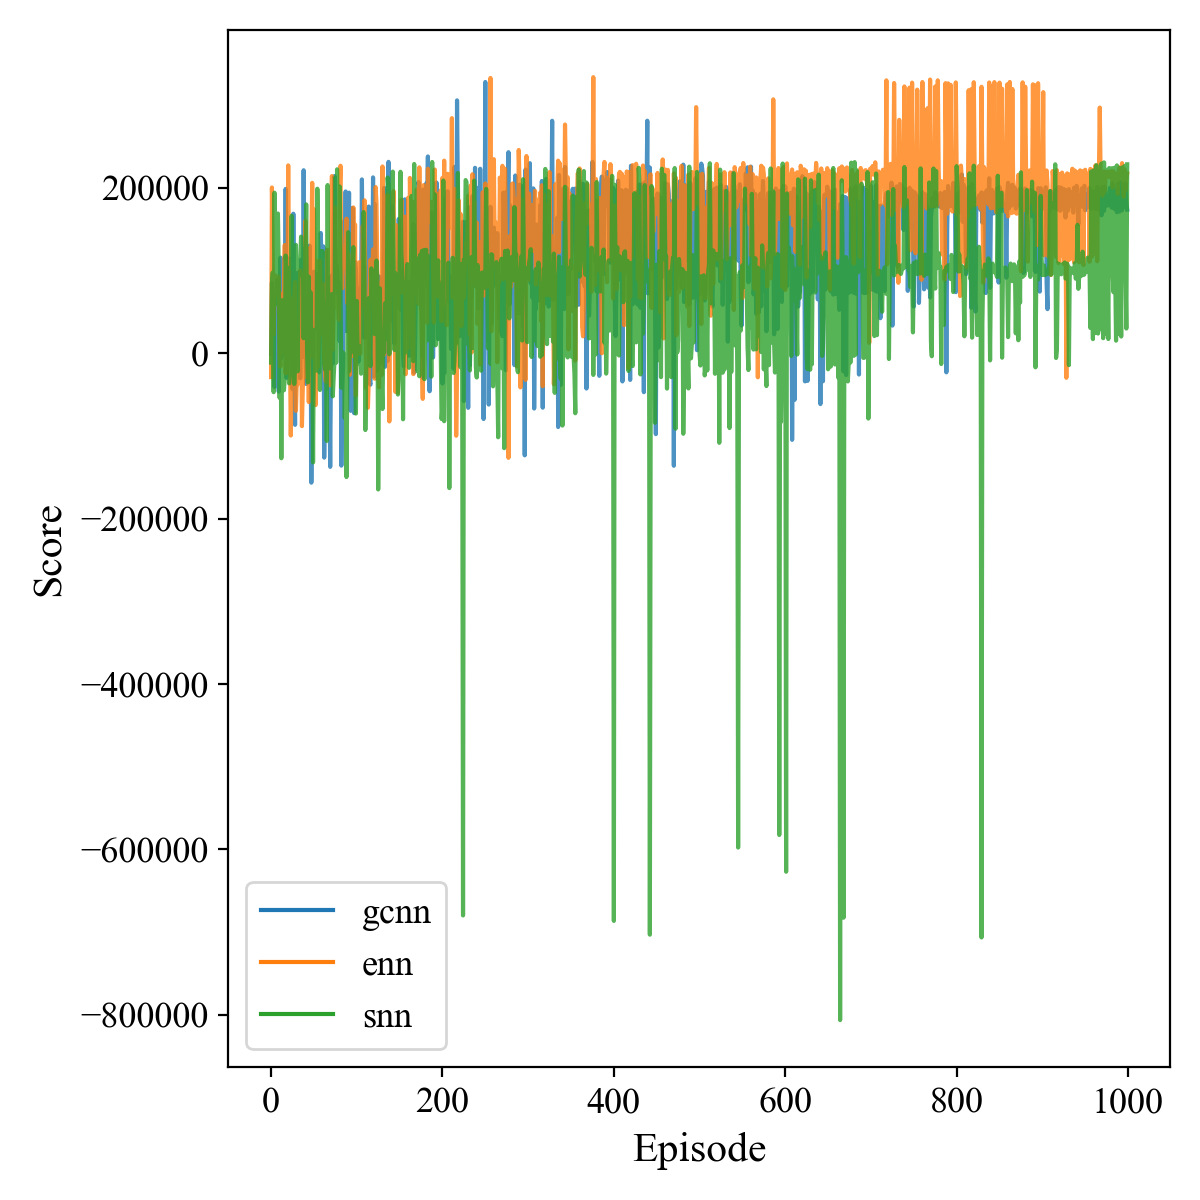
\includegraphics[width=6.5cm, keepaspectratio]{images/scores_history_comparison_test_5_intersection}<1>	
	
	\only<2>{Smoothed with 50-size window (mixed mode)}	
	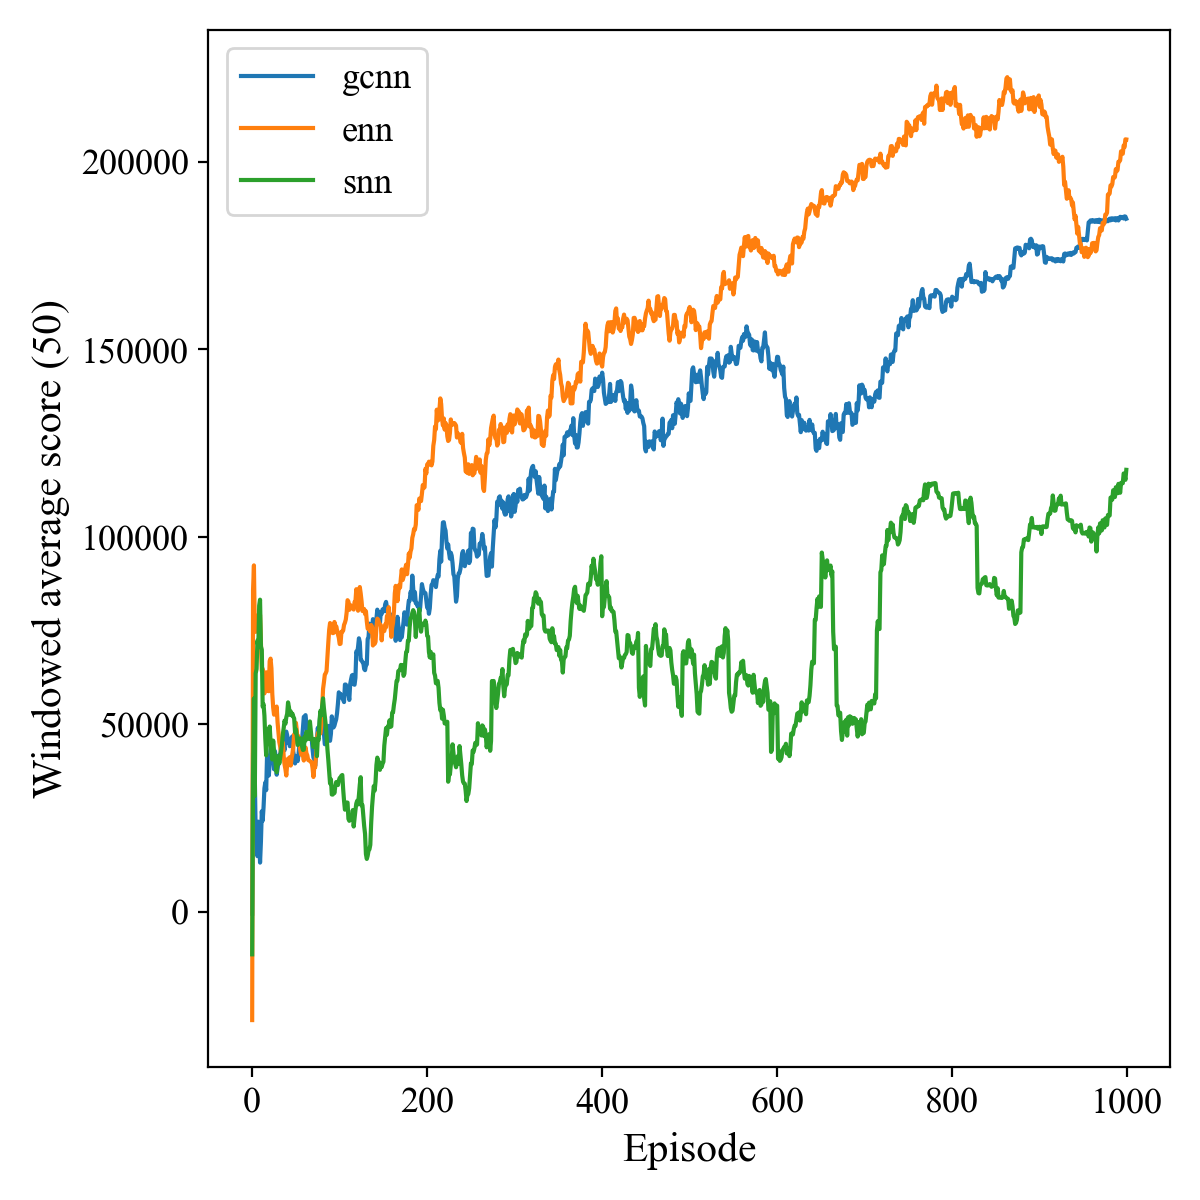
\includegraphics[width=6.5cm, keepaspectratio]{images/windowed_scores_comparison_test_5_intersection}<2>	
	
	\only<3>{Total averages (mixed mode)}	
	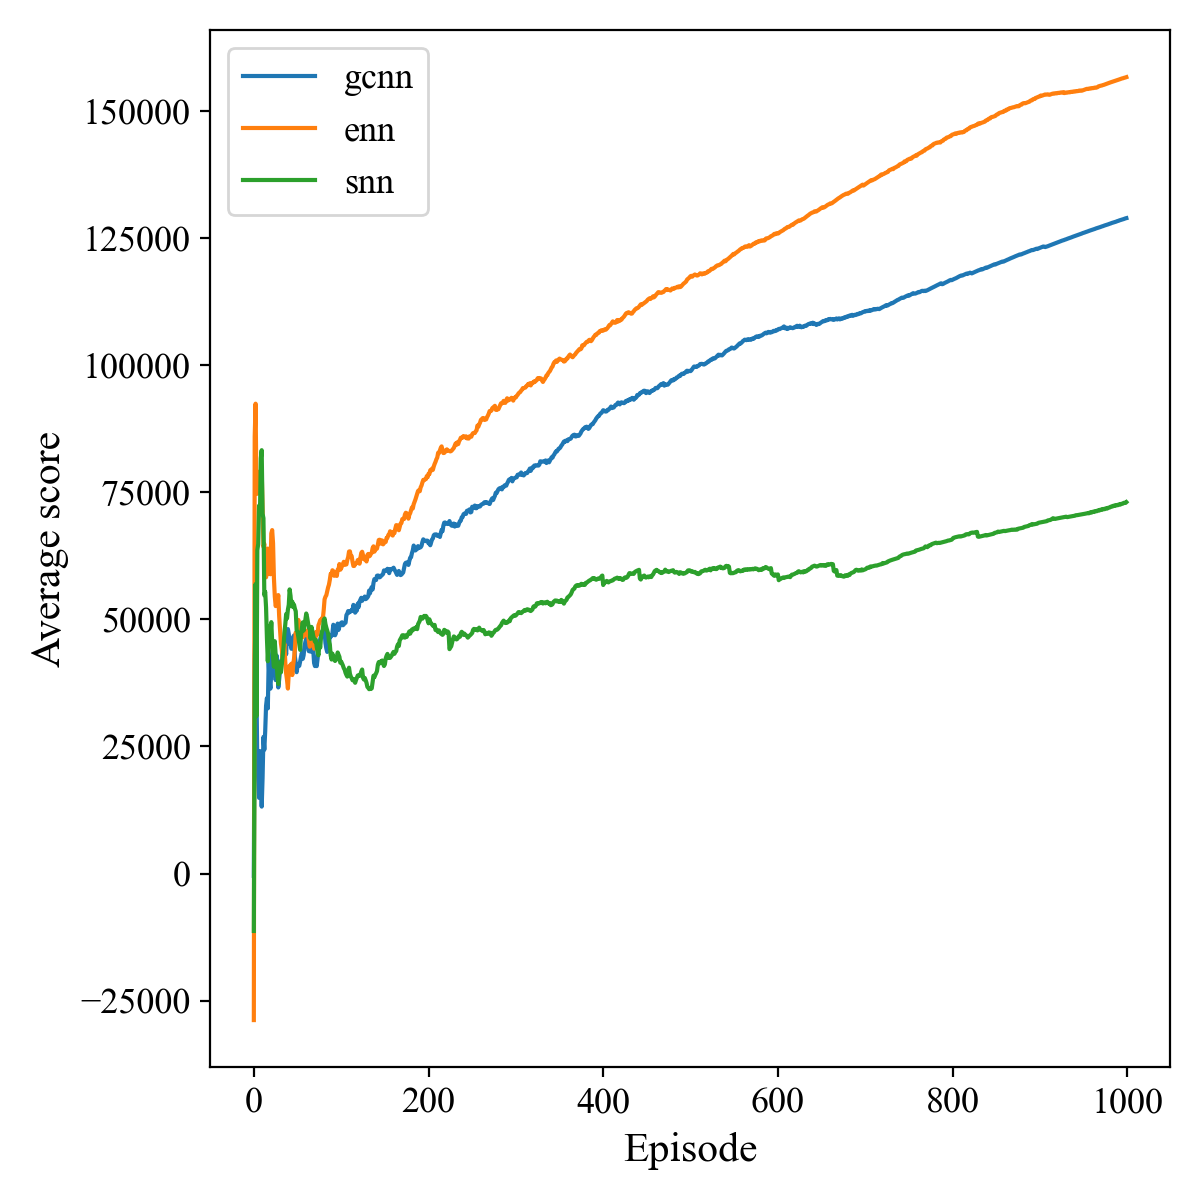
\includegraphics[width=6.5cm, keepaspectratio]{images/average_scores_comparison_test_5_intersection}<3>	
			
	\only<4>{Unsmoothed rewards (green-field mode)}	
	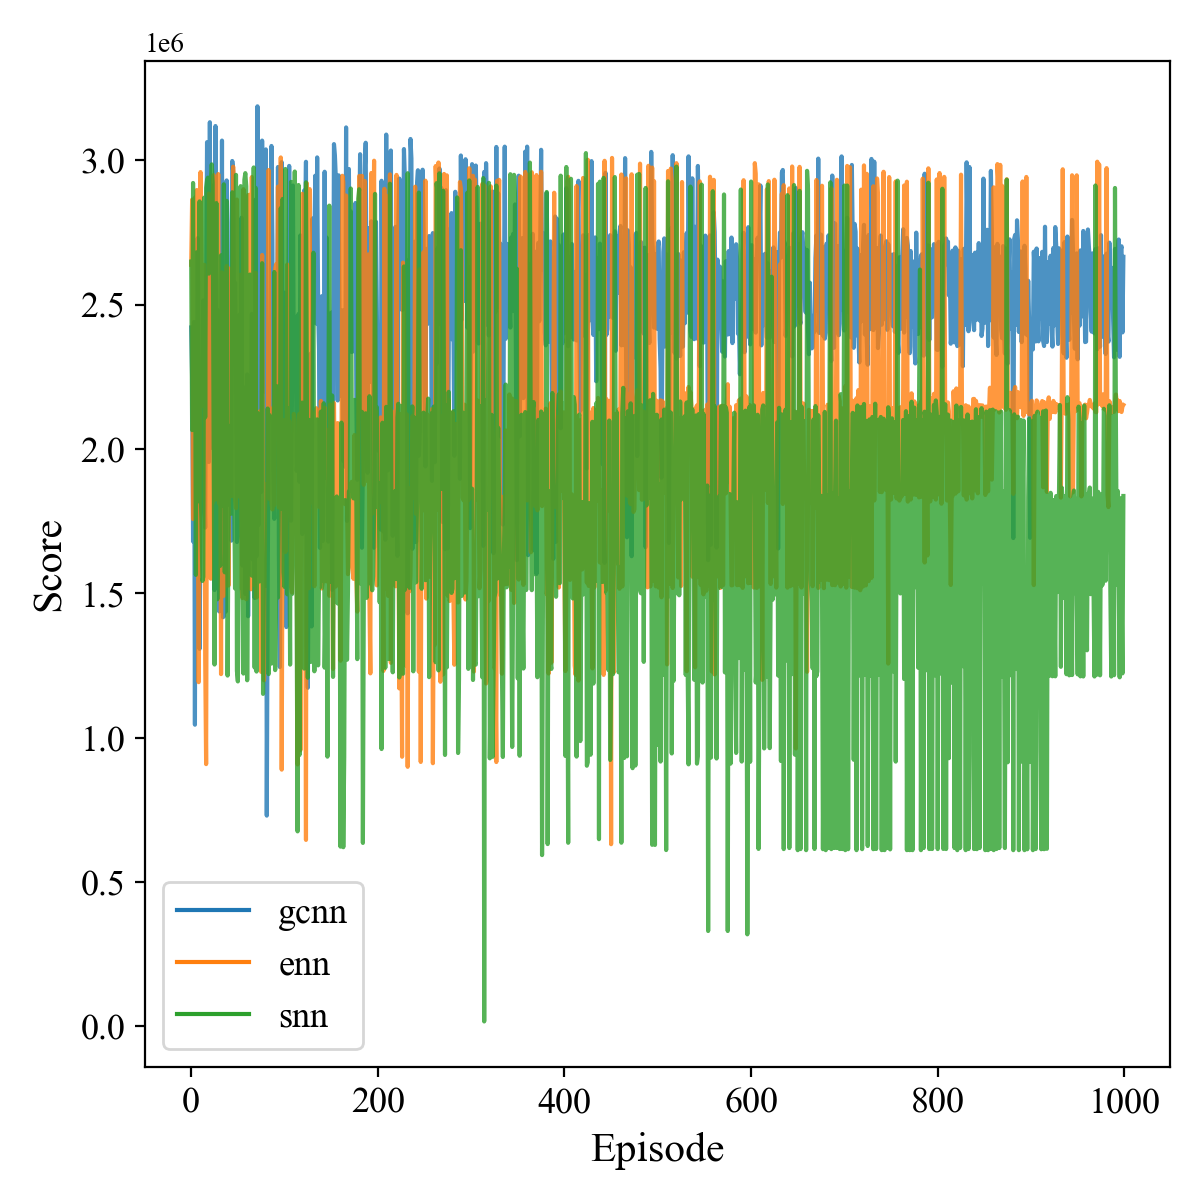
\includegraphics[width=6.5cm, keepaspectratio]{images/scores_history_comparison_test_5_intersection_empty}<4>	
	
	\only<5>{Smoothed with 50-size window (green-field mode)}	
	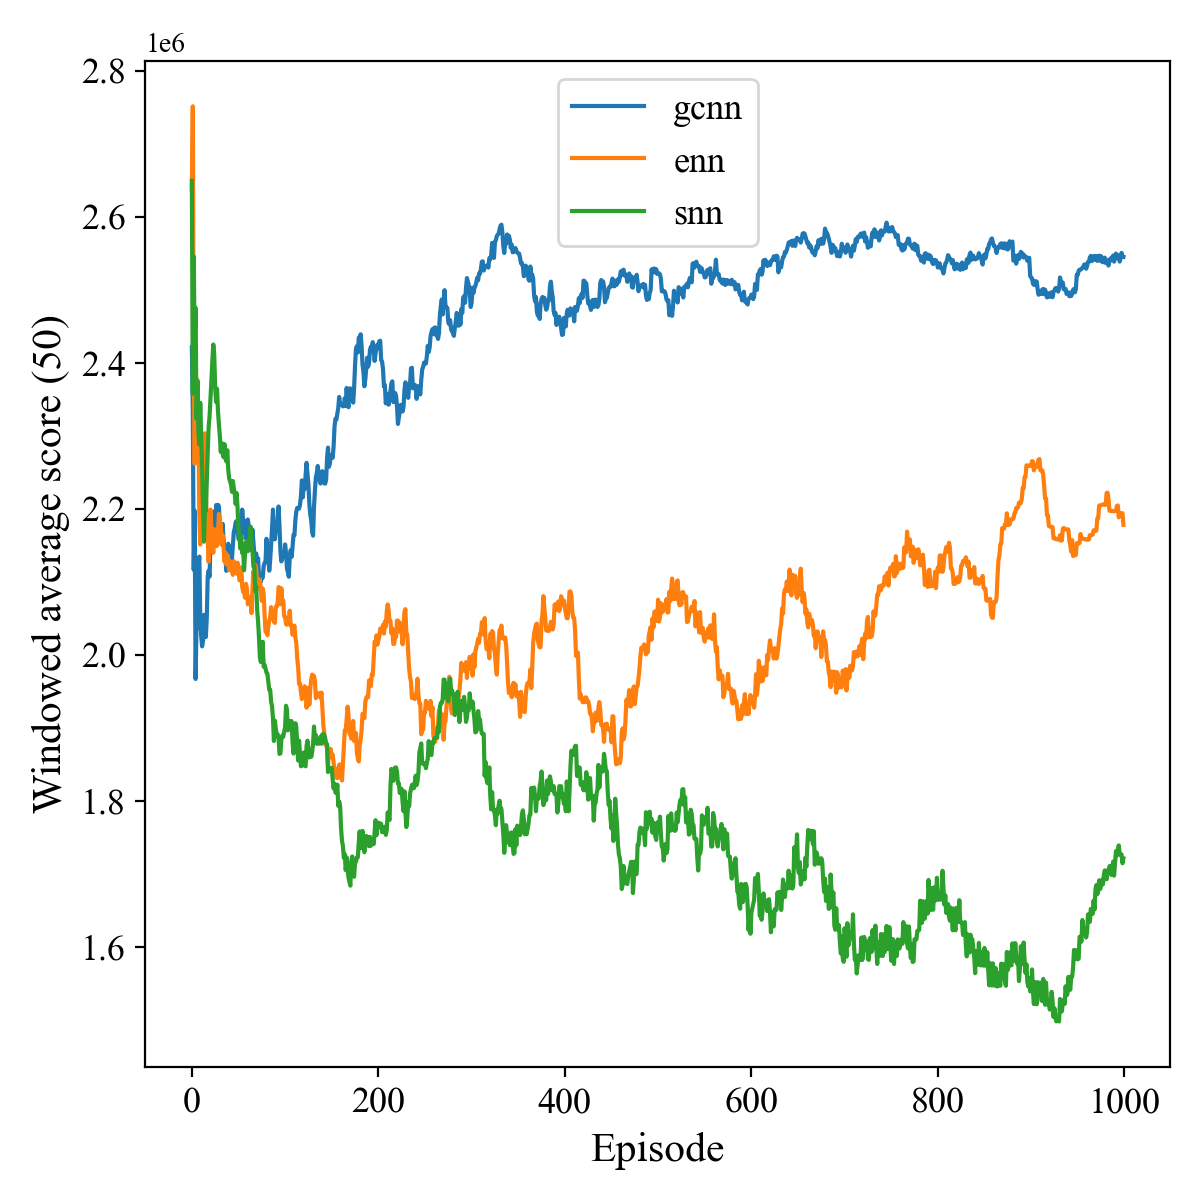
\includegraphics[width=6.5cm, keepaspectratio]{images/windowed_scores_comparison_test_5_intersection_empty}<5>	
	
	\only<6>{Total averages (green-field mode)}	
	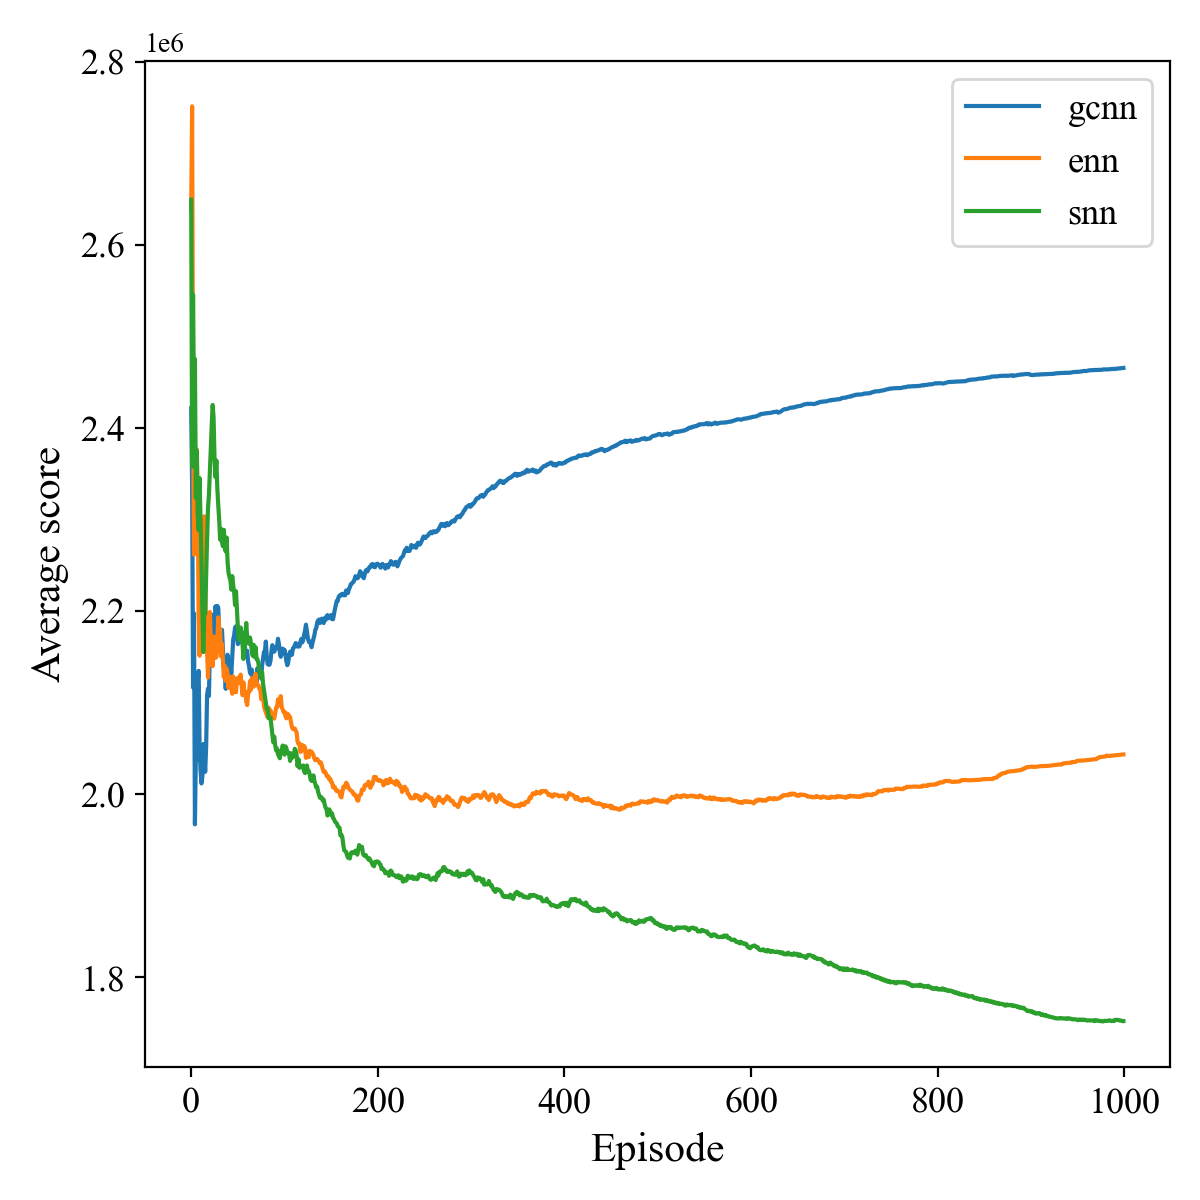
\includegraphics[width=6.5cm, keepaspectratio]{images/average_scores_comparison_test_5_intersection_empty}<6>				
			
	\end{scriptsize}
	
	\end{center}

\end{column}

\end{columns}
\end{frame}

\subsection{Cities designed by the agents}

\begin{frame}{Cities built by the agent}
\begin{columns}[T]

\begin{column}{0.5\textwidth}
	After the learning episodes the agent was used to execute 15 building steps in the environment. 
	\begin{itemize}
		\only<1->{\item Graph-convolutional model (mixed)}
		\only<2->{\item Graph-convolutional model (green-field)}
		\only<3->{\item Embedding-based model (mixed)}
		\only<4->{\item Embedding-based model (green-field)}
		\only<5->{\item Adjacency matrix-based model (mixed)}
		\only<6->{\item Adjacency matrix-model (green-field)}
	\end{itemize}
\end{column}

\begin{column}{0.5\textwidth}
	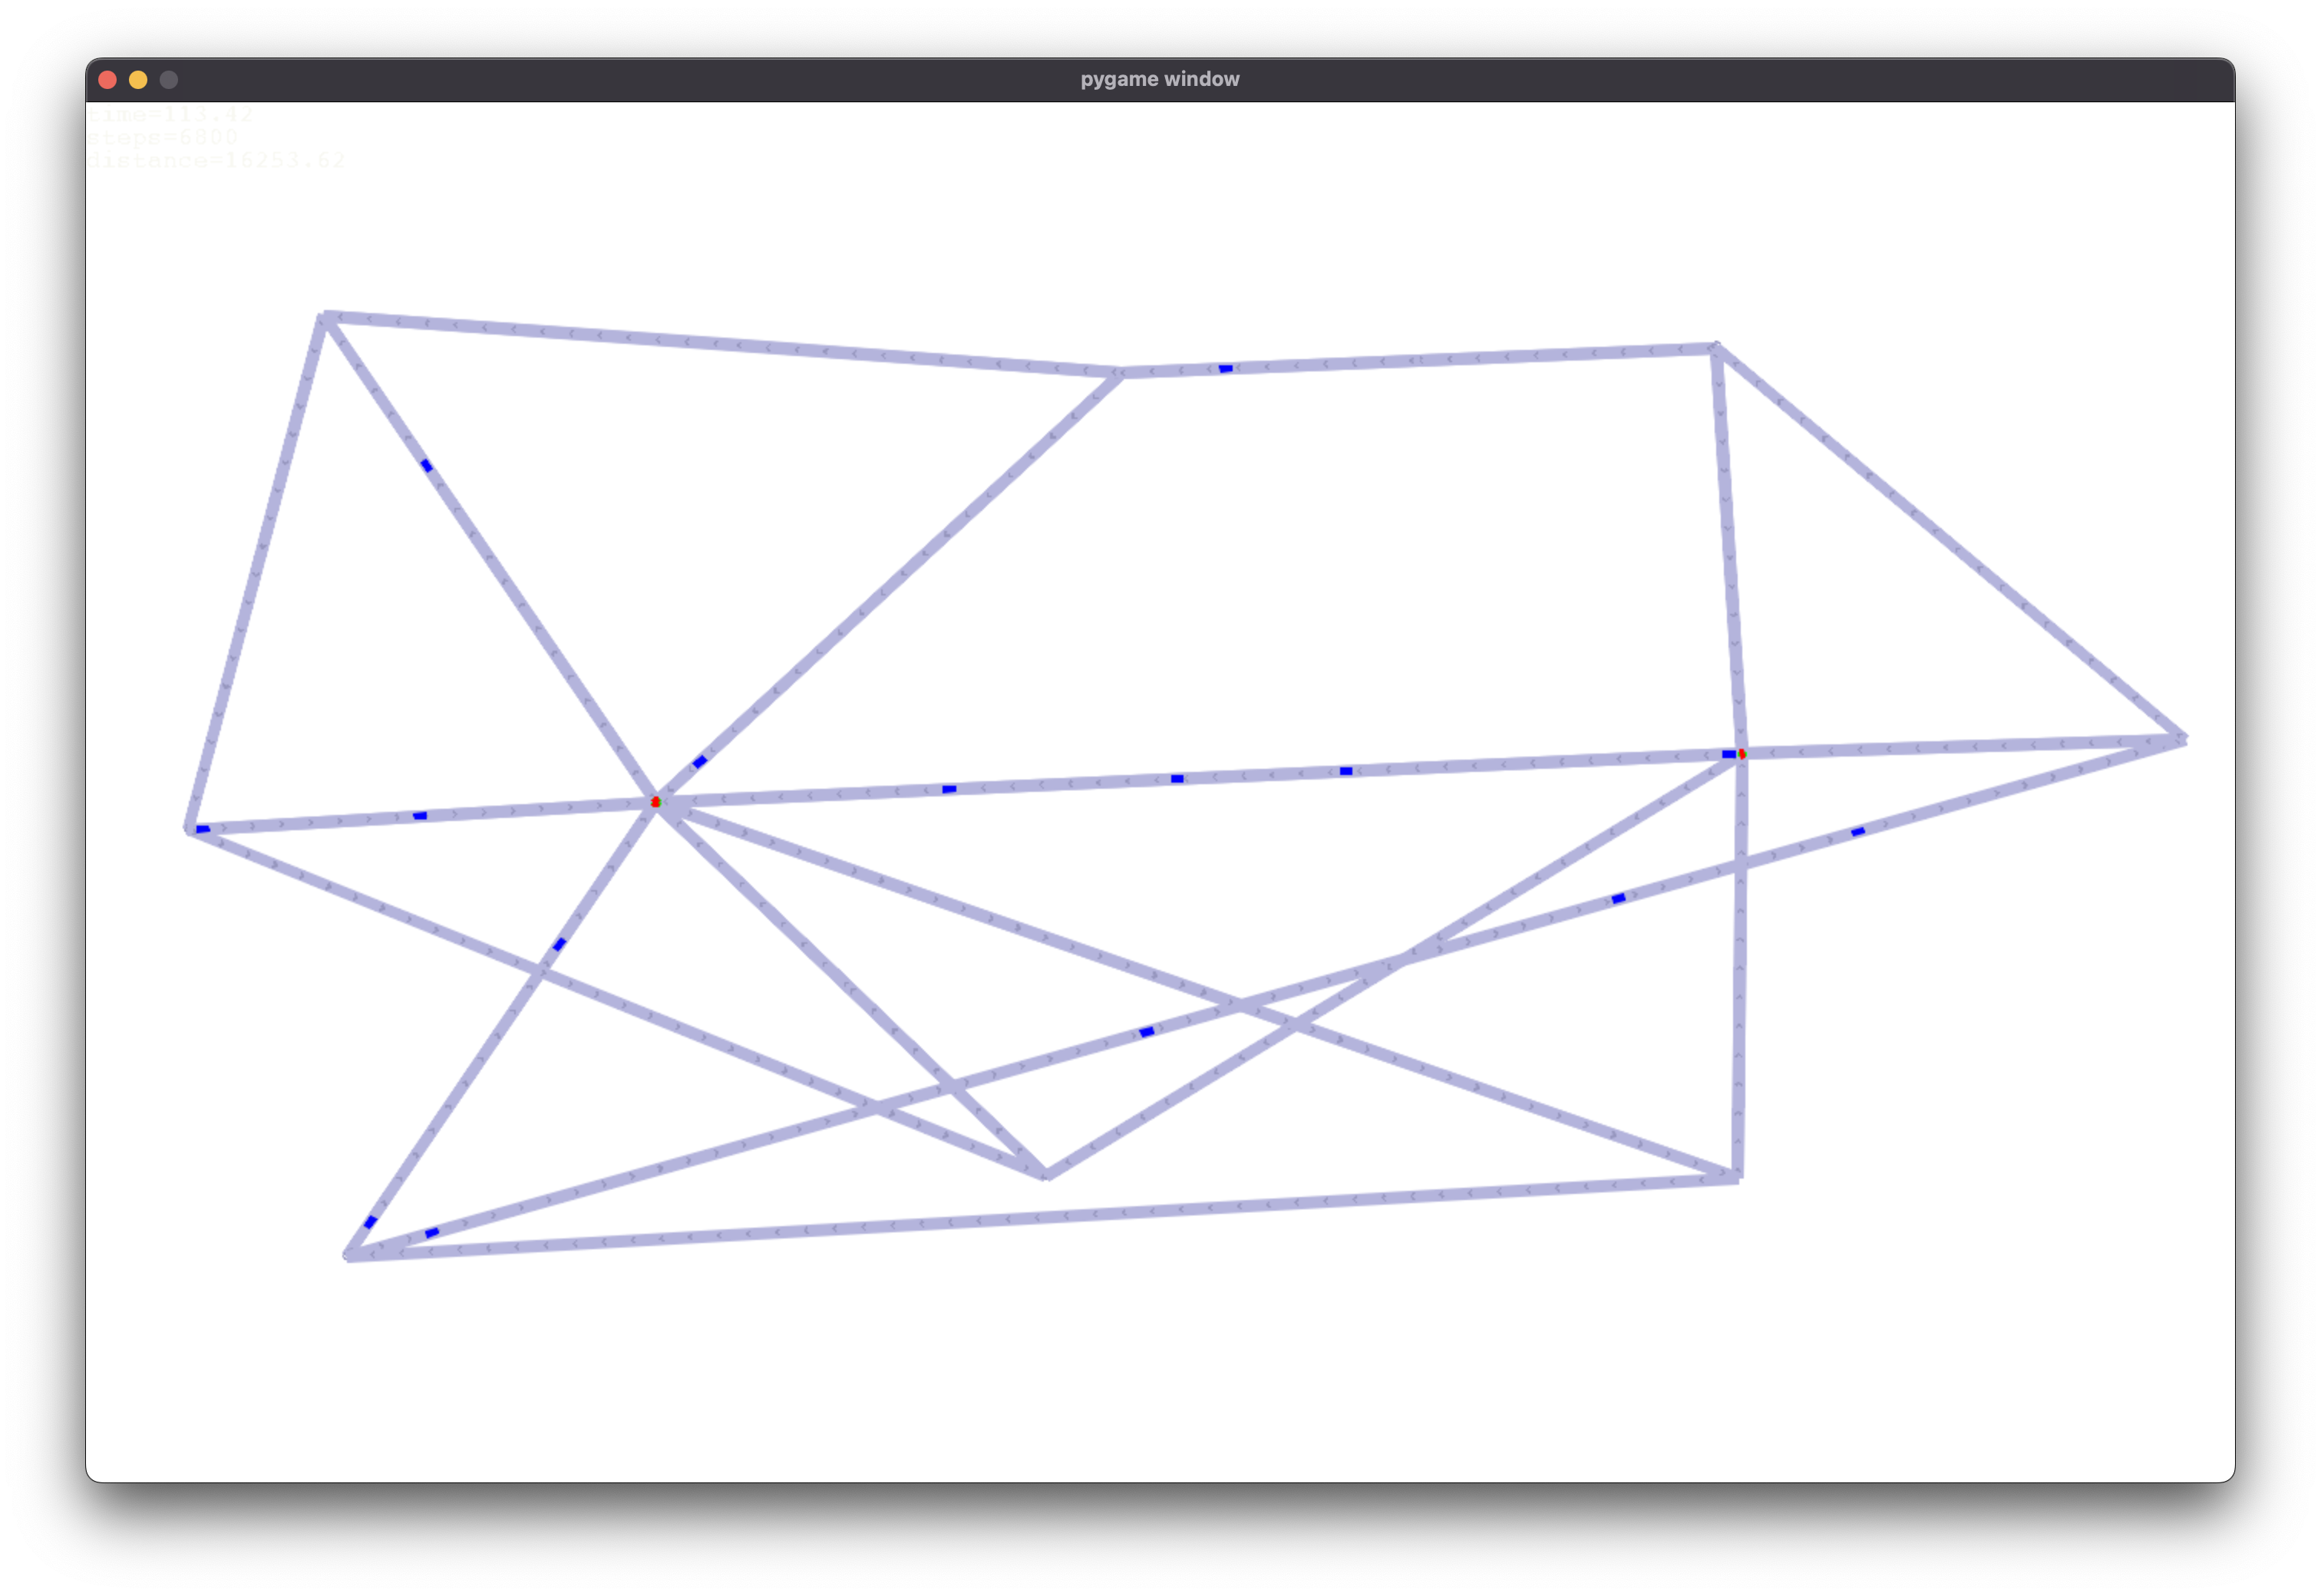
\includegraphics[width=7cm, height=7cm, keepaspectratio]{images/city_agent_gcnn_2023-05-03_23-33_test_5_intersection}<1>
	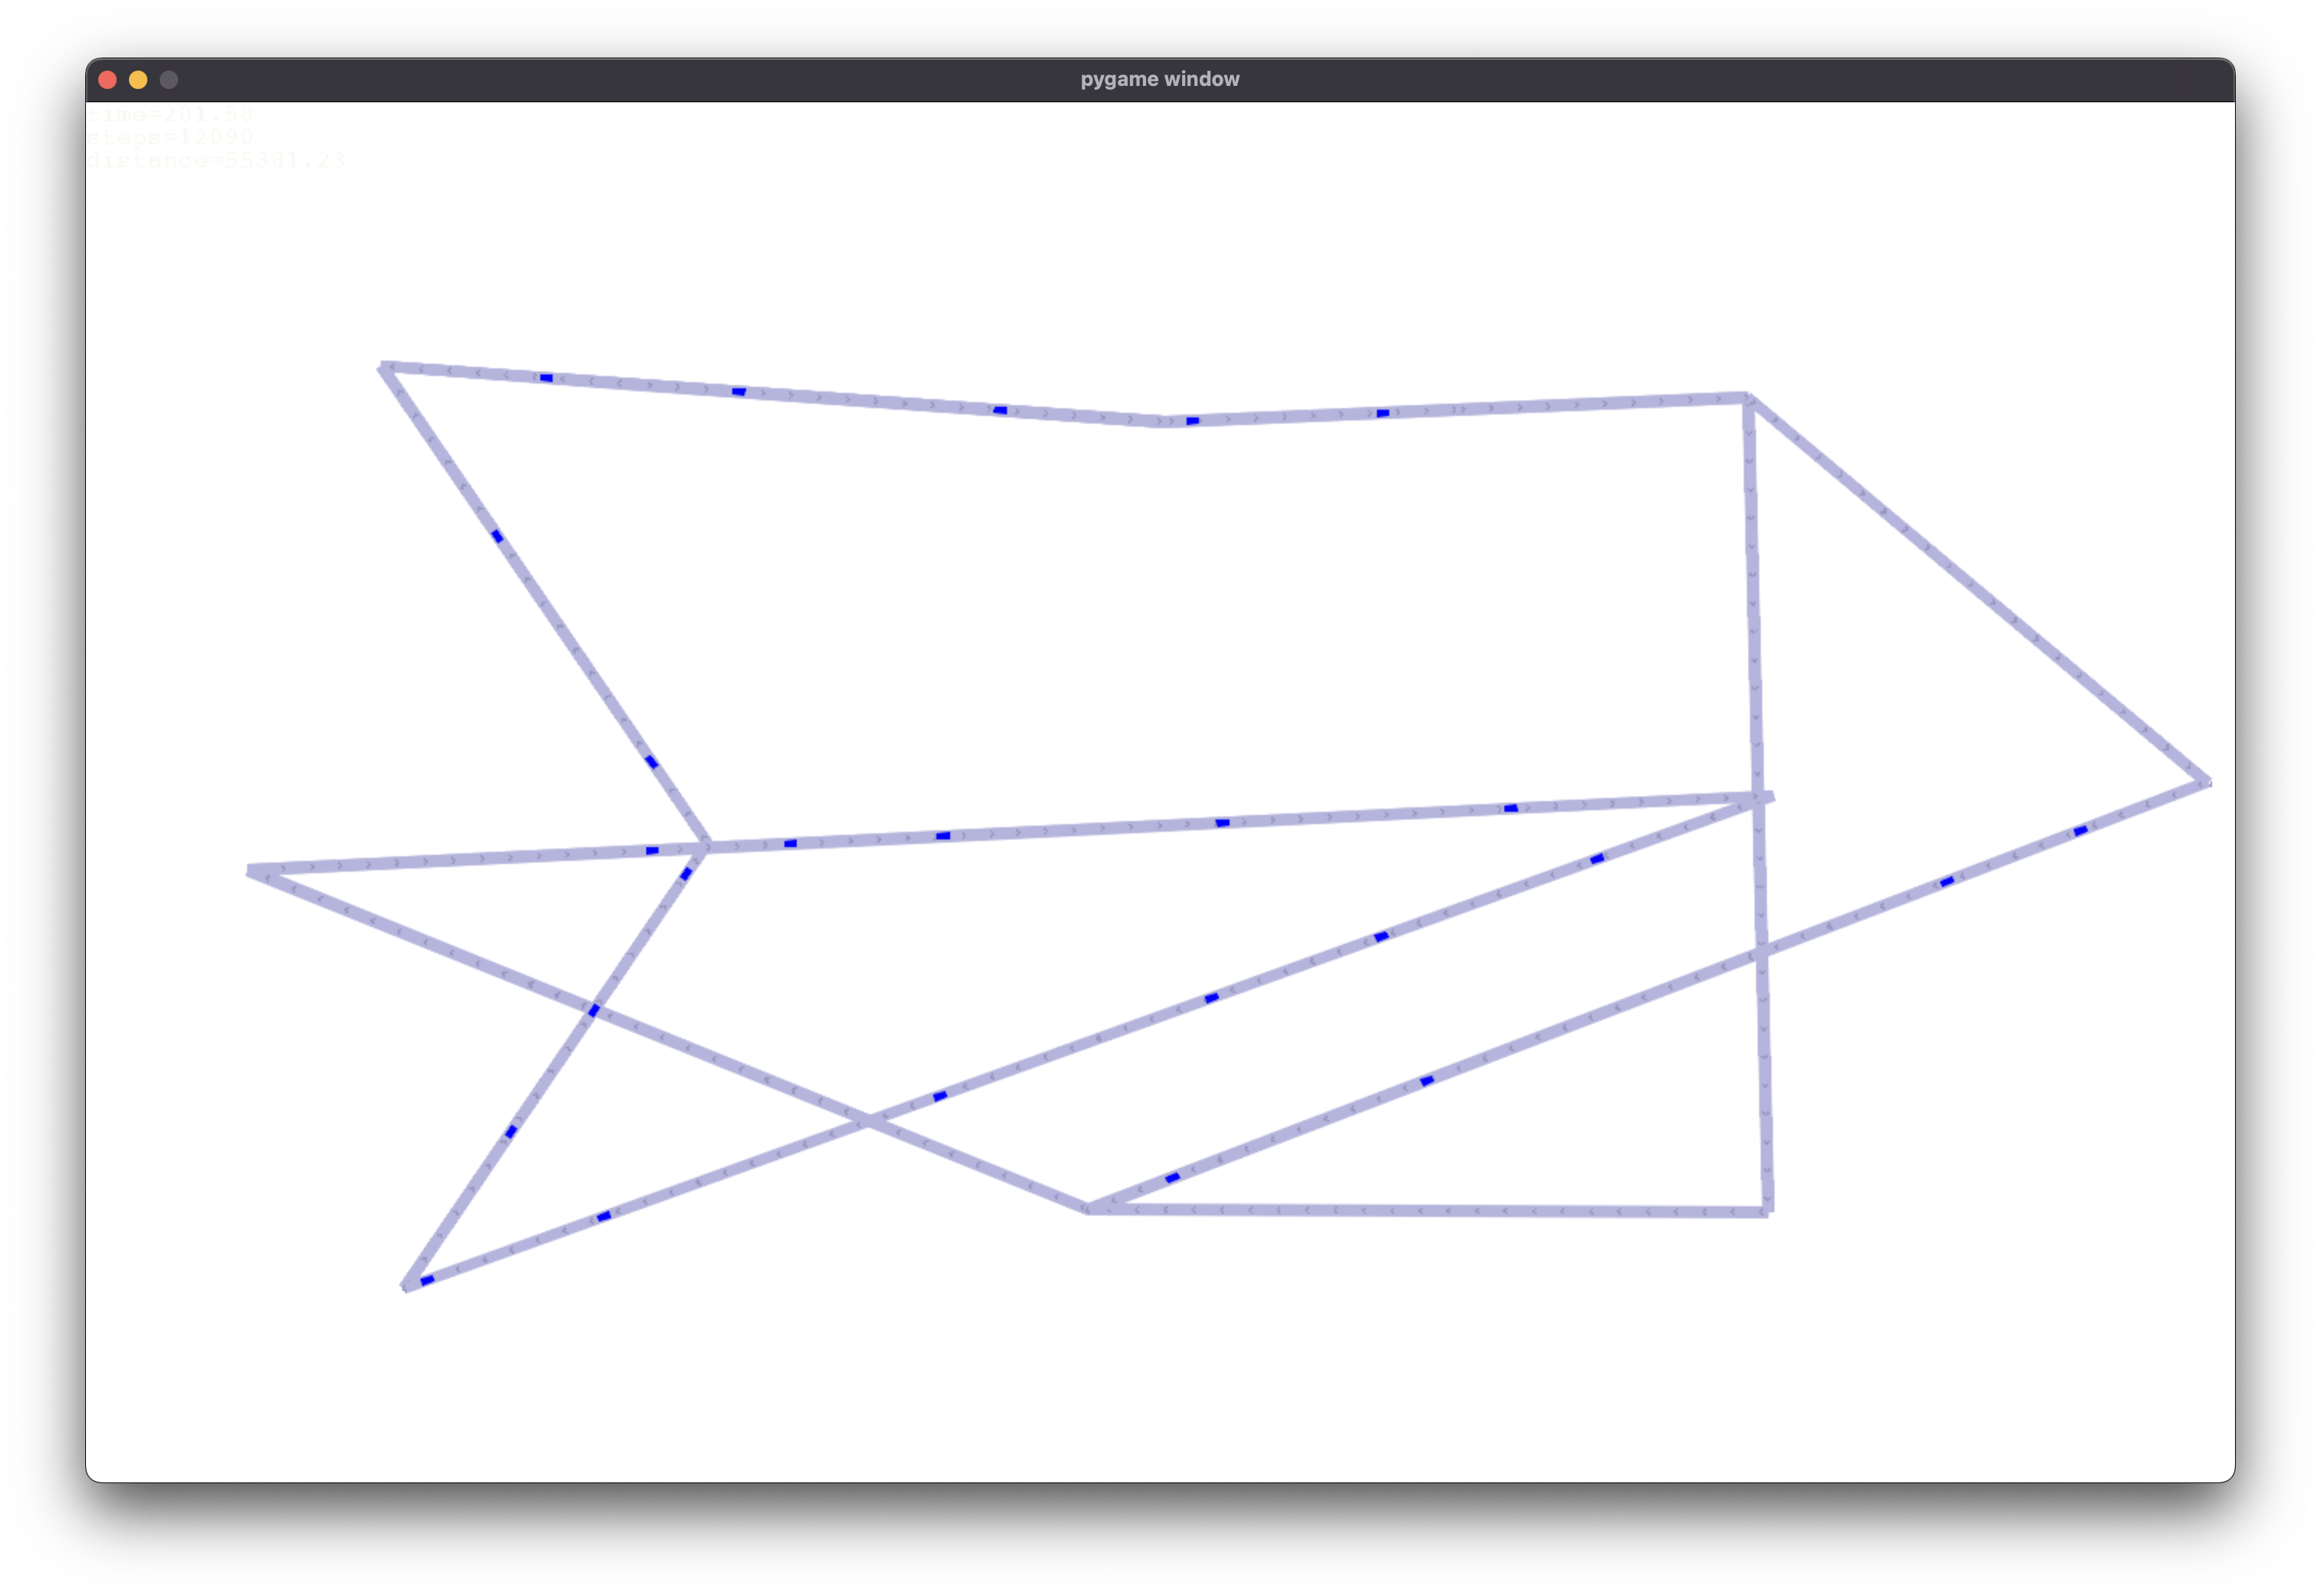
\includegraphics[width=7cm, height=7cm, keepaspectratio]{images/city_agent_gcnn_2023-04-29_18-06_test_5_intersection_empty}<2>
	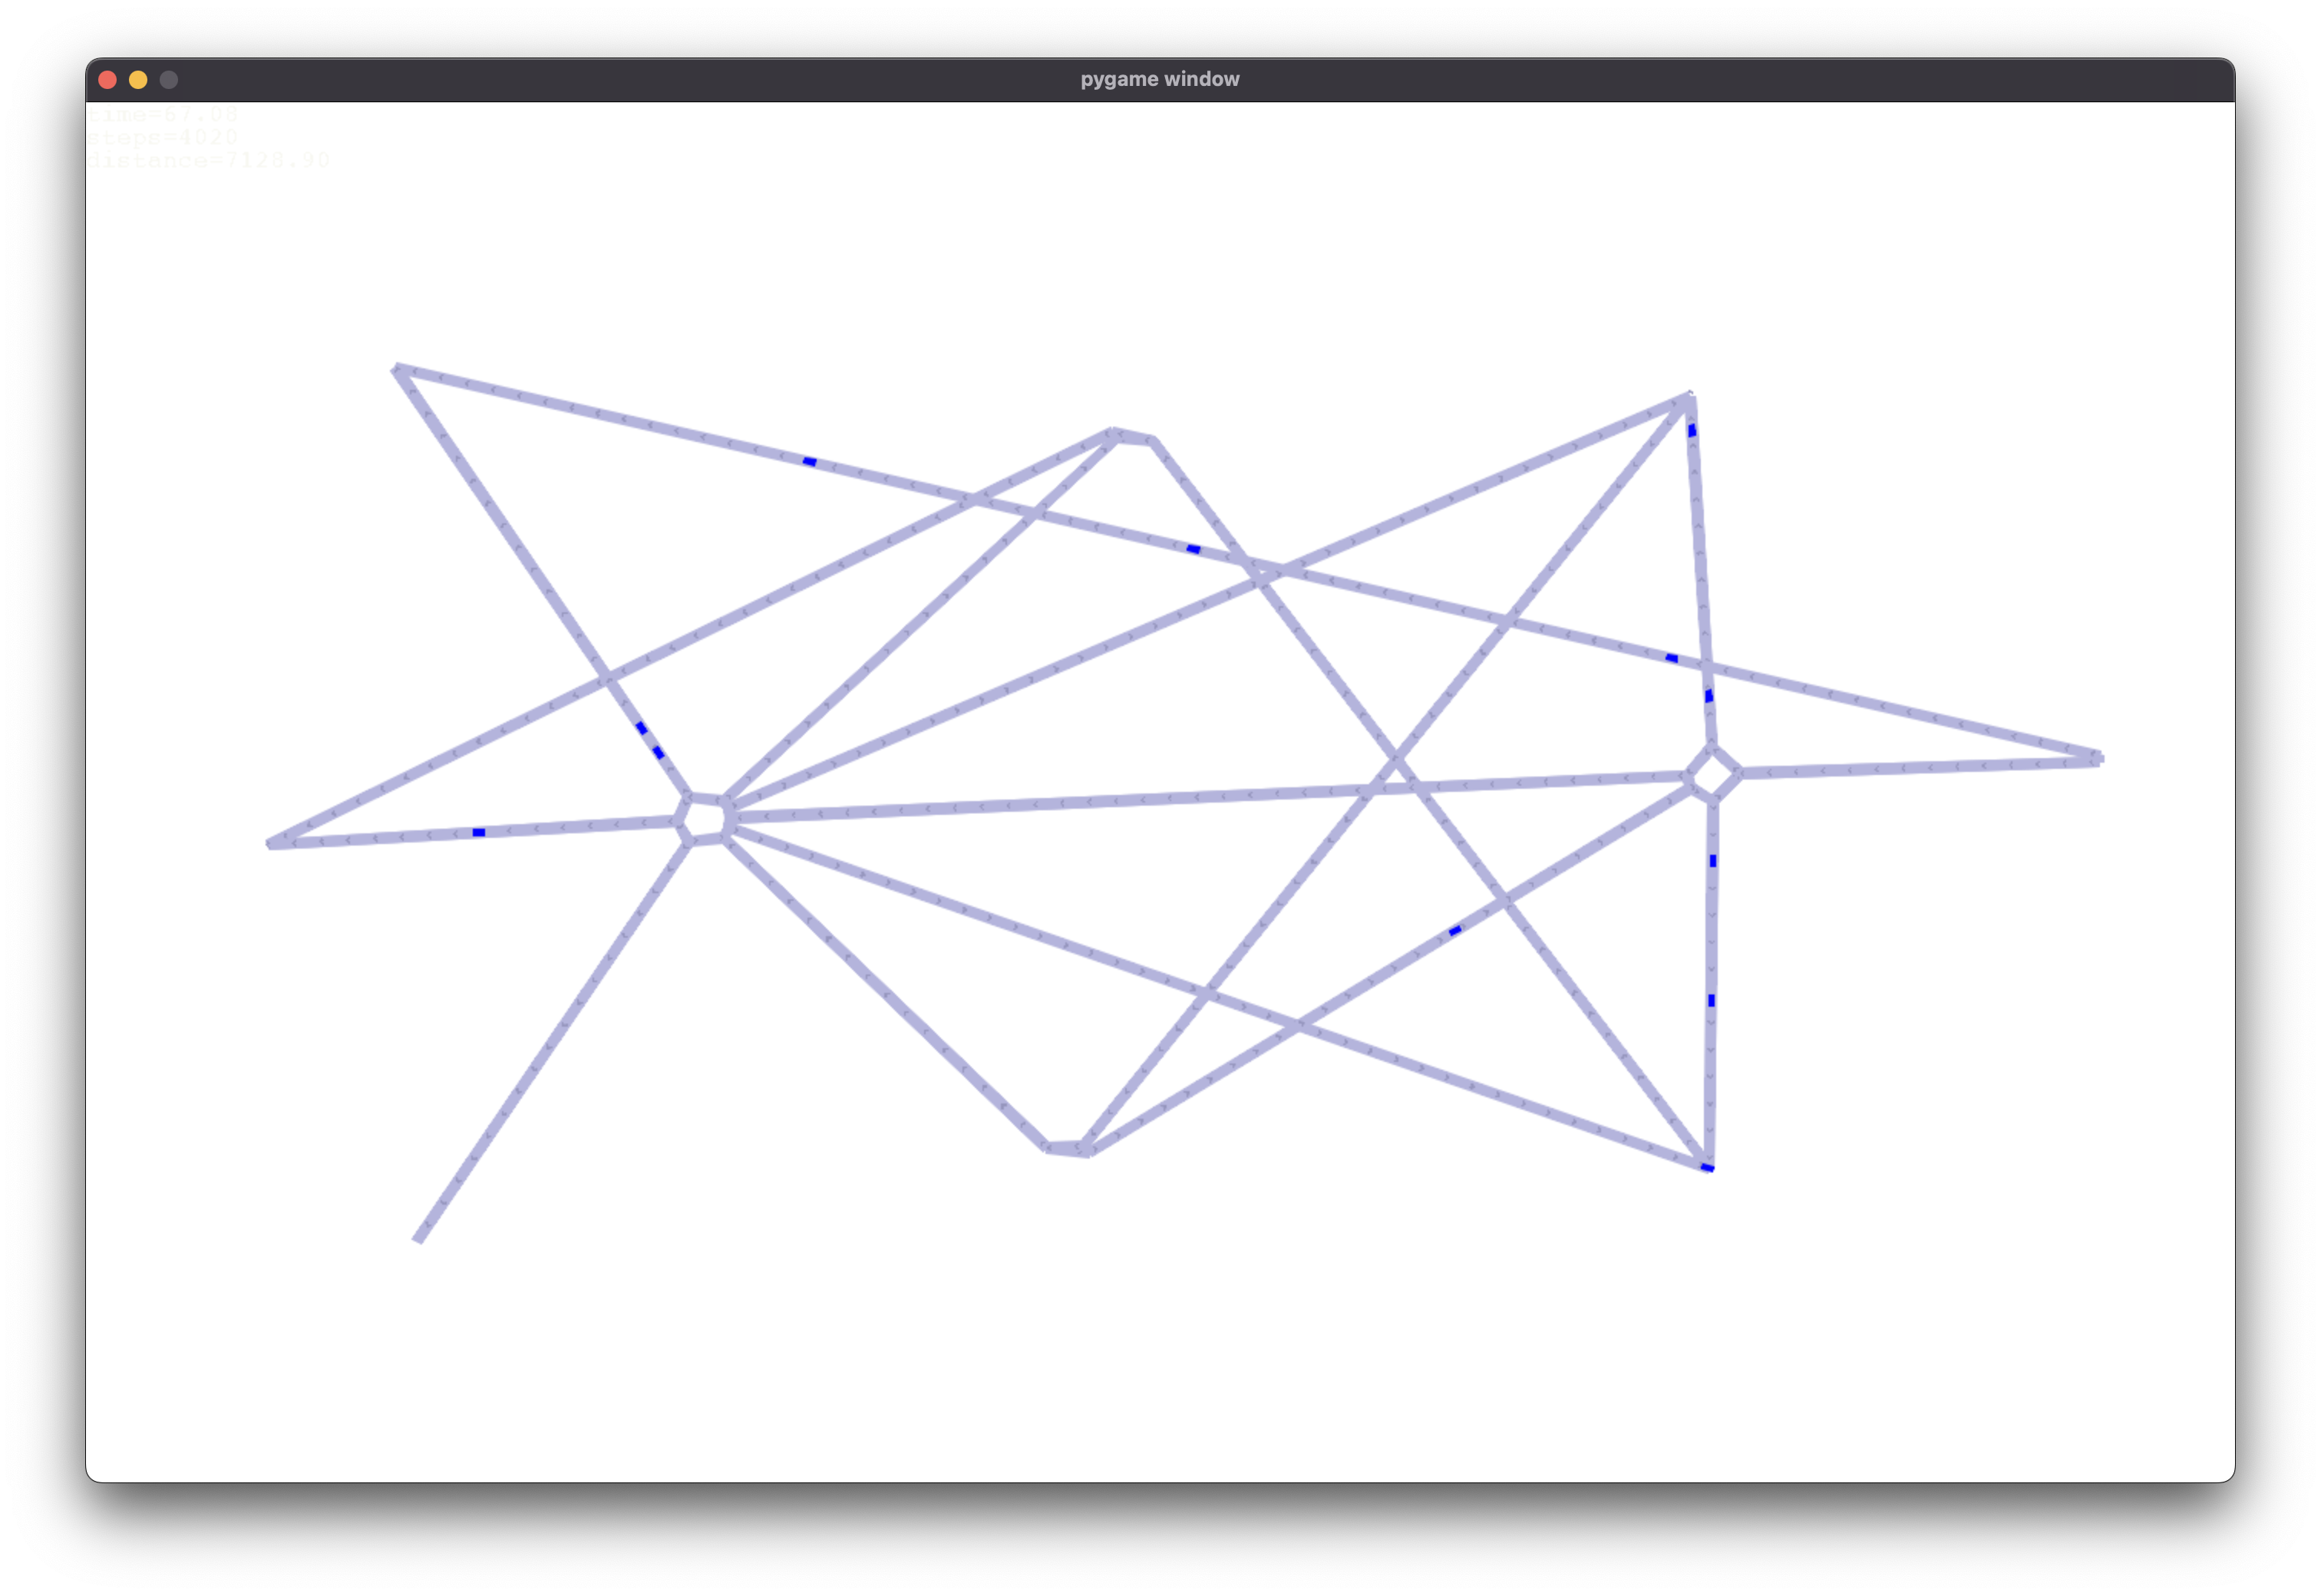
\includegraphics[width=7cm, height=7cm, keepaspectratio]{images/city_agent_enn_2023-05-04_10-53_test_5_intersection}<3>
	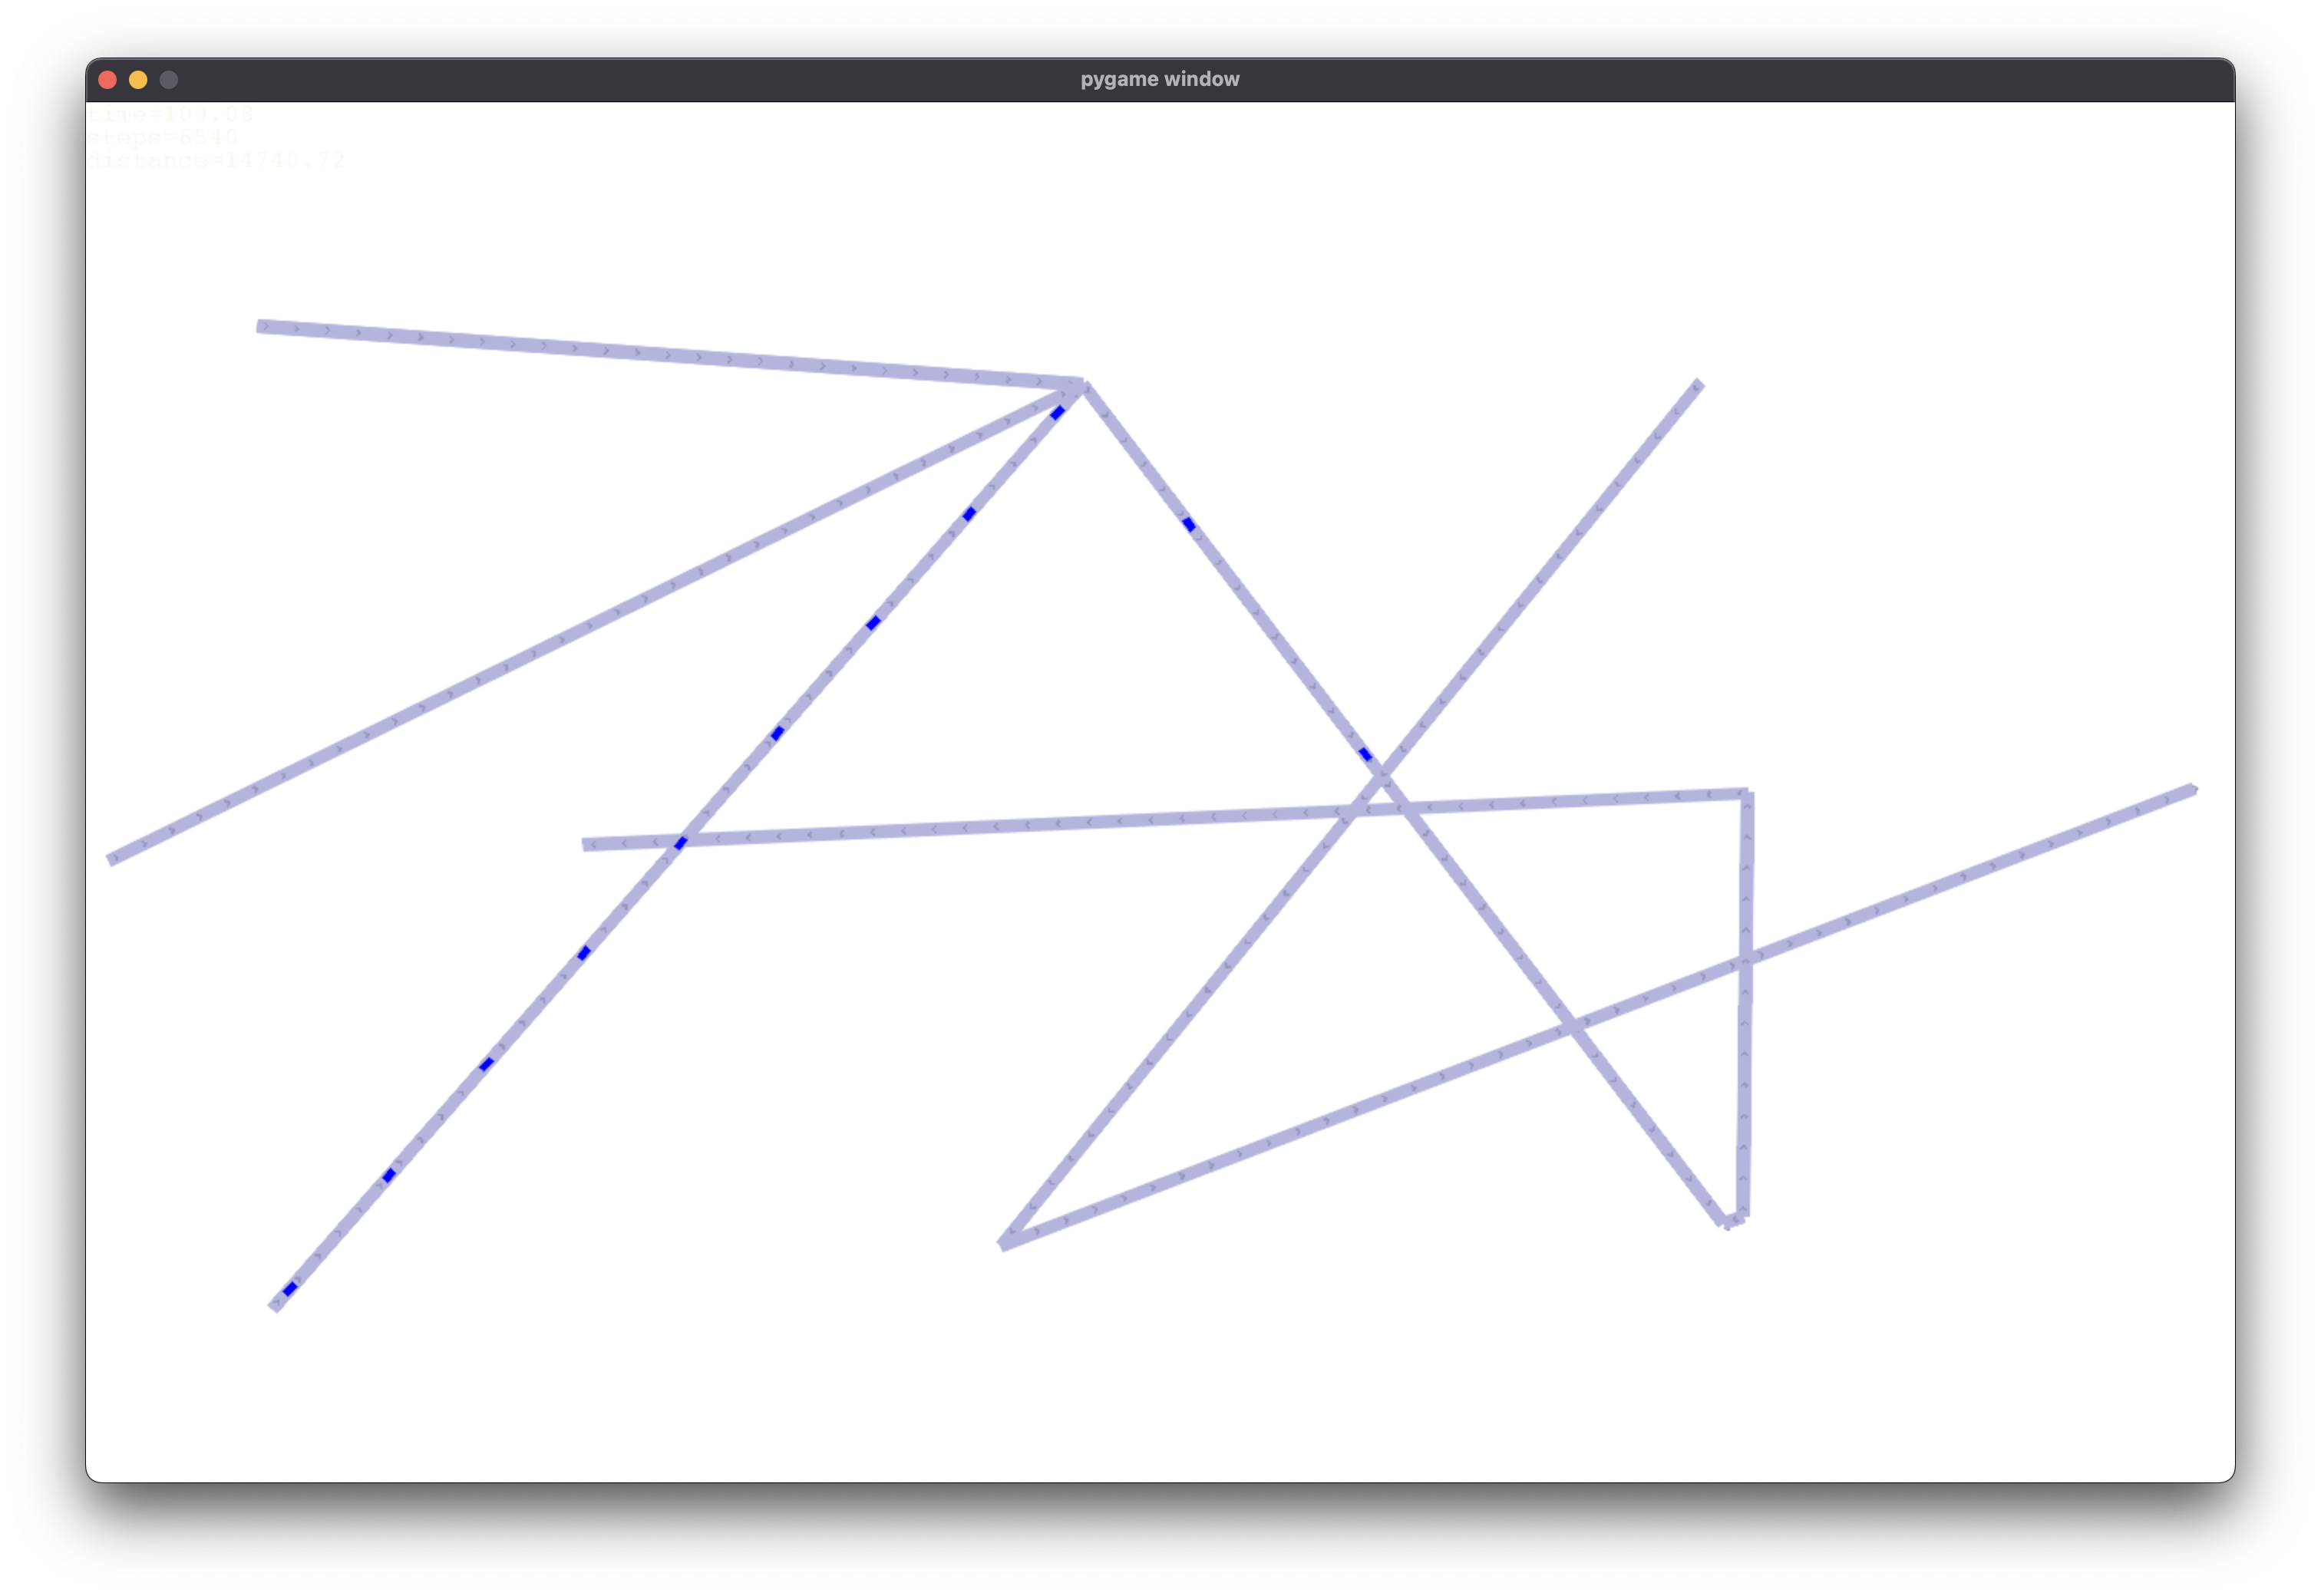
\includegraphics[width=7cm, height=7cm, keepaspectratio]{images/city_agent_enn_2023-05-04_22-59_test_5_intersection_empty}<4>
	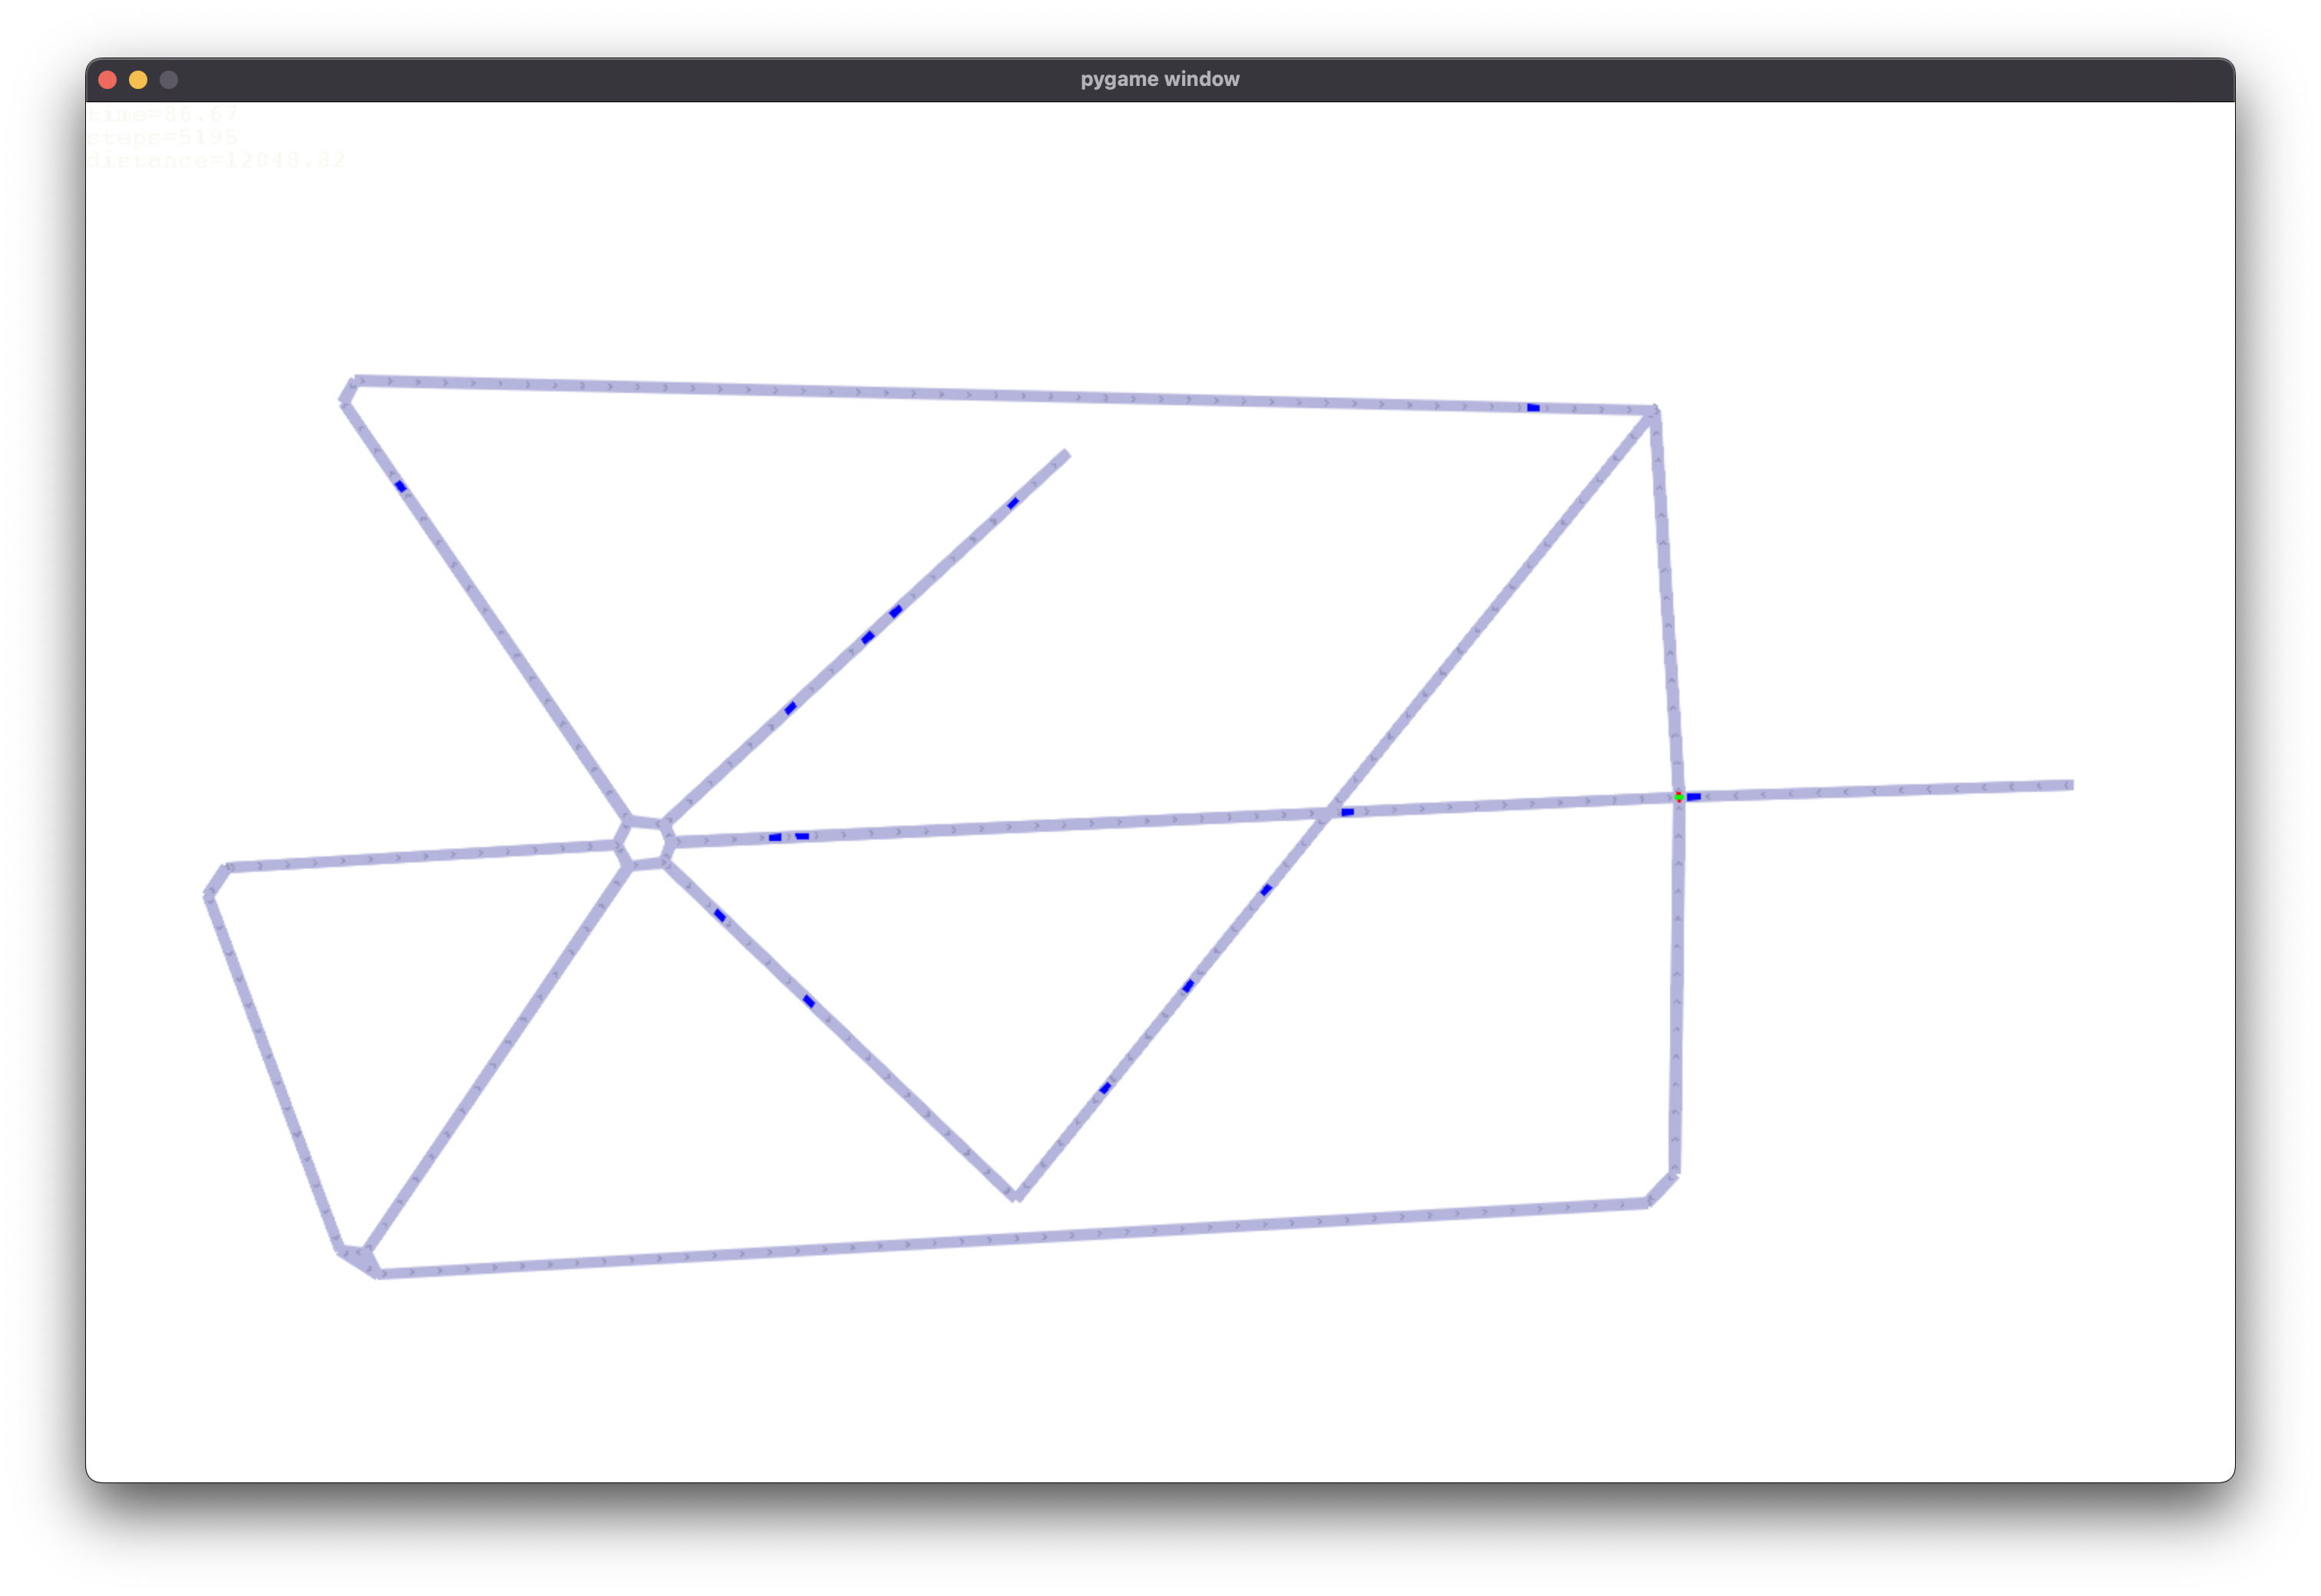
\includegraphics[width=7cm, height=7cm, keepaspectratio]{images/city_agent_snn_2023-05-04_14-28_test_5_intersection}<5>
	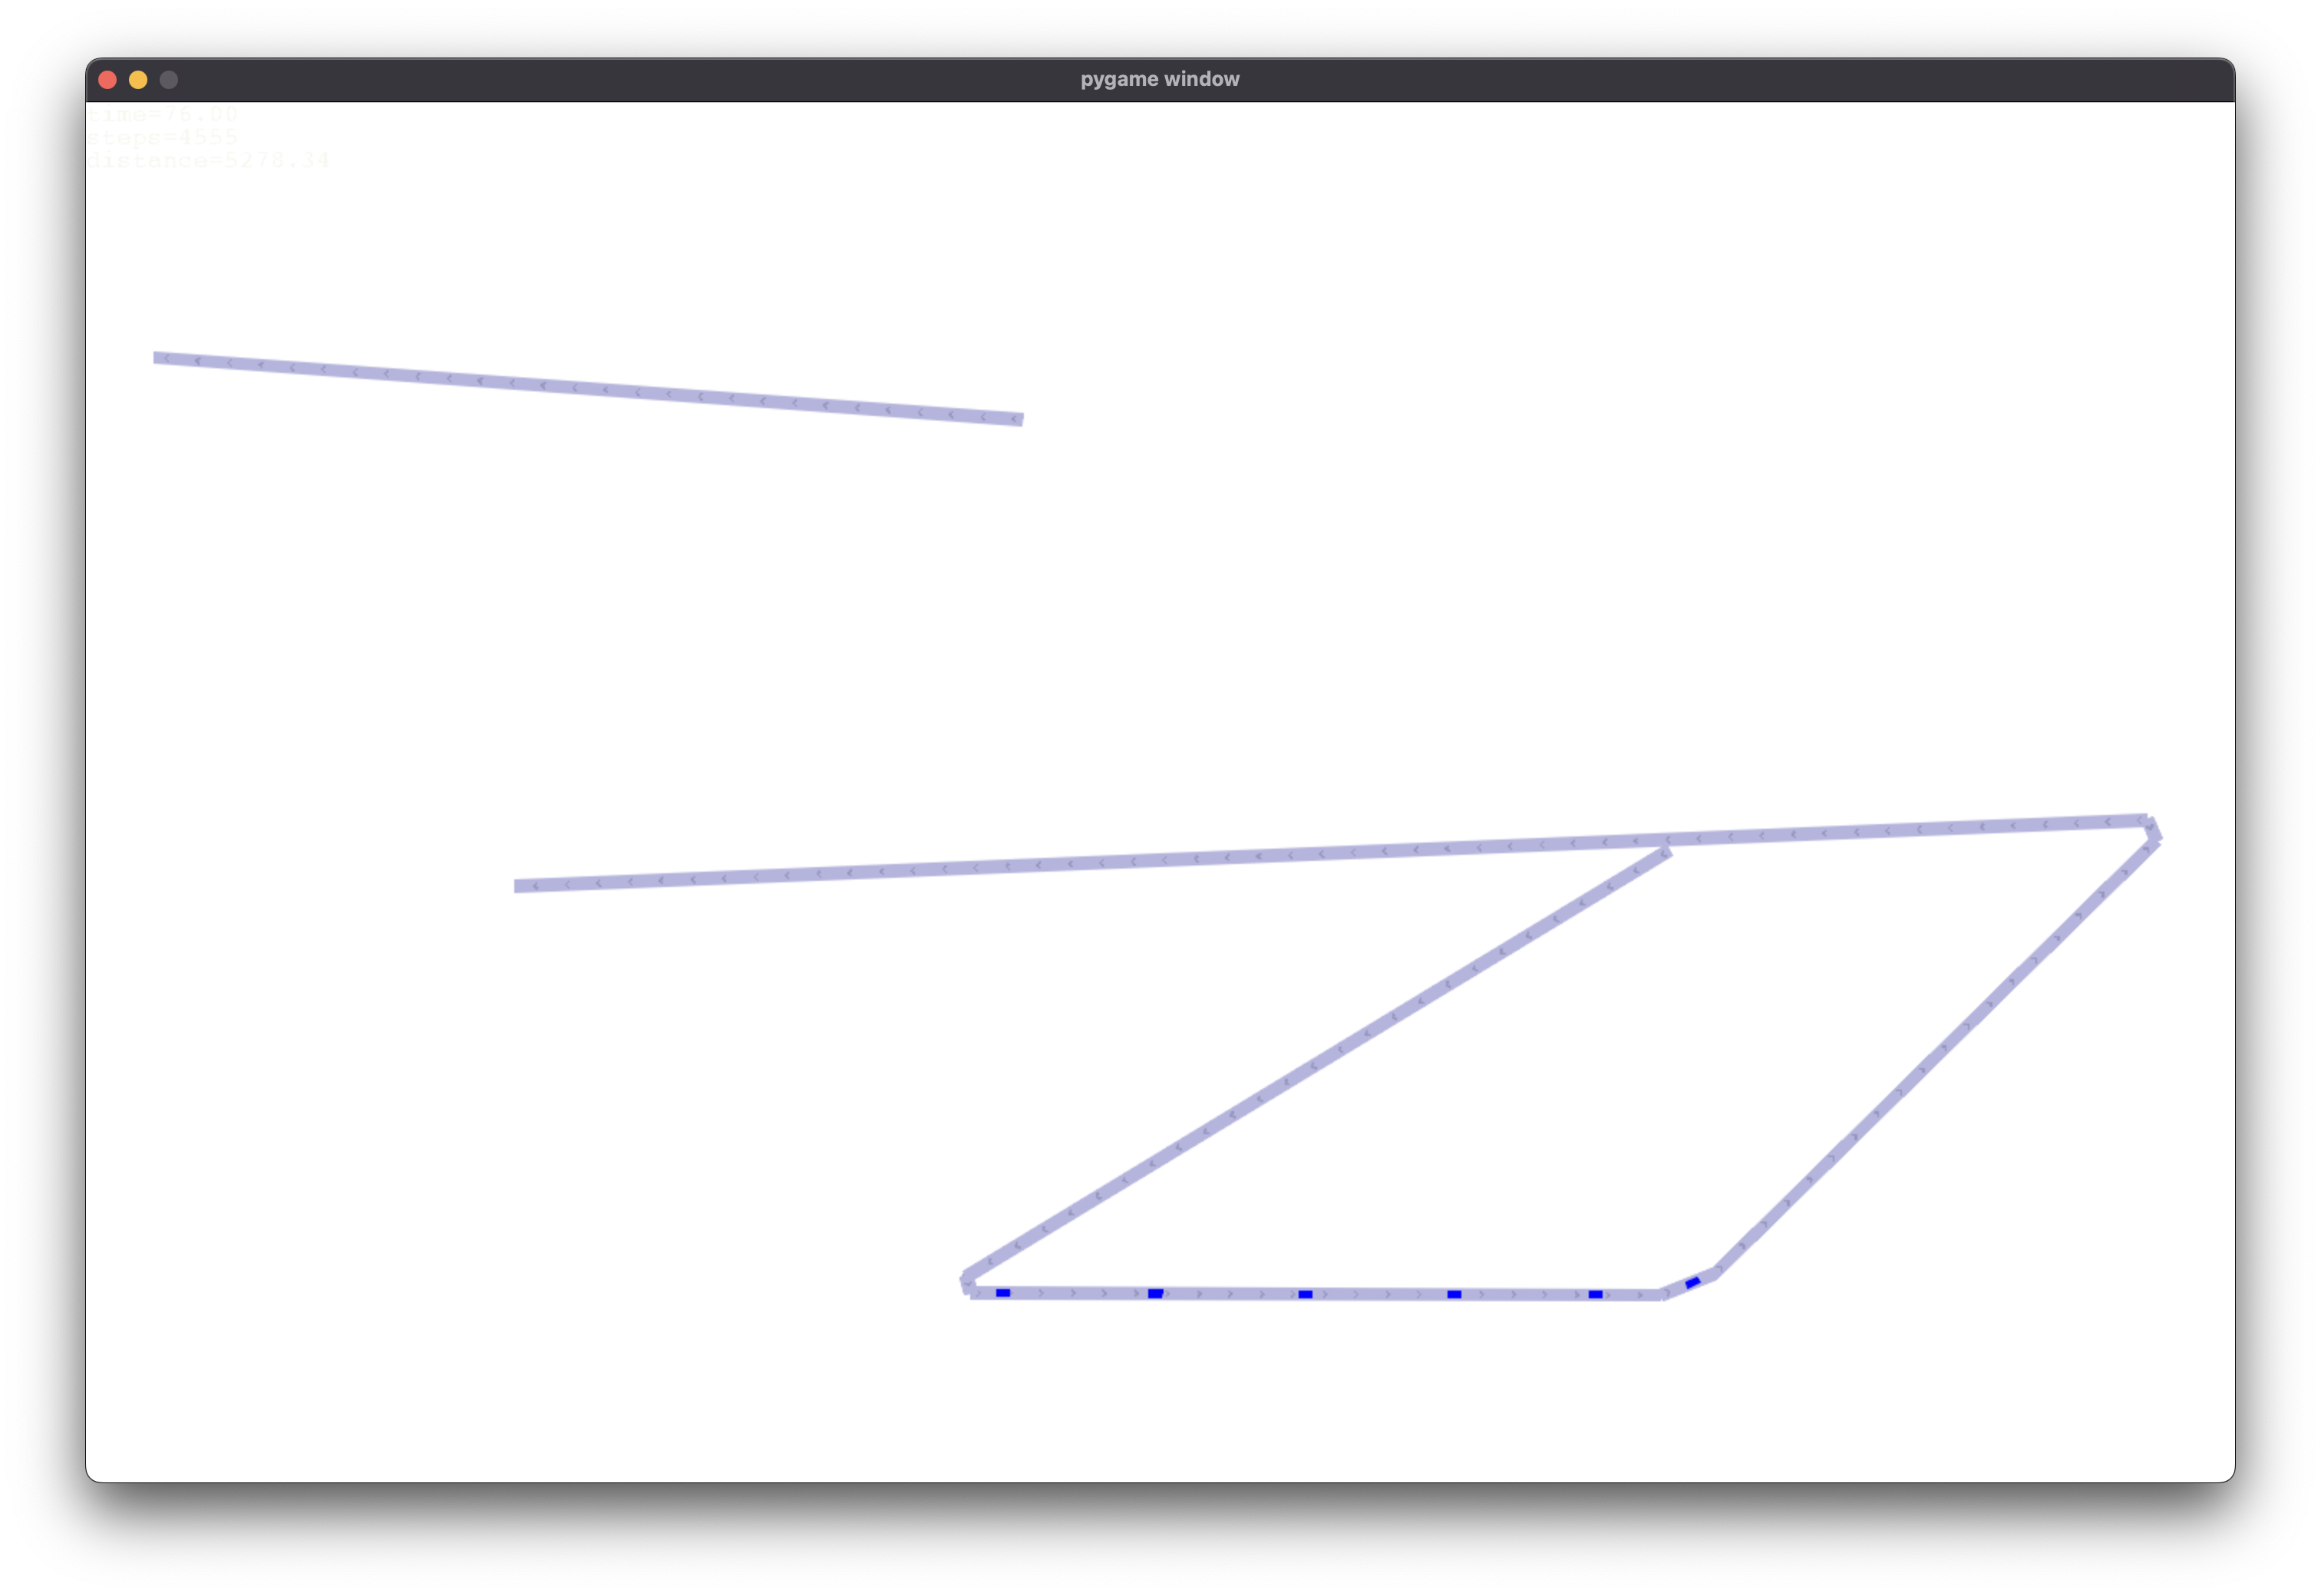
\includegraphics[width=7cm, height=7cm, keepaspectratio]{images/city_agent_snn_2023-05-04_20-30_test_5_intersection_empty}<6>
	
	
	\begin{itemize}
	\begin{small}
		\only<1>{\item Distant nodes were connected}
		\only<1>{\item Traffic lights added on central junctions}
		\only<1>{\item Fast traffic flow and humanly livable}
		
		\only<2>{\item Distant nodes were connected}
		\only<2>{\item No traffic lights or roundabouts}
		\only<2>{\item Road structure doesn't allow smooth flow}		
		
		\only<3>{\item Fully optimized for cars}
		\only<3>{\item Roundabouts in central junctions}
		\only<3>{\item Fast traffic flow but not human-friendly}
		
		\only<4>{\item The traffic system is not continuous}
		\only<4>{\item No junction is left without a connection}
		\only<4>{\item No roundabouts or traffic lights}
		
		\only<5>{\item Distant nodes were connected}
		\only<5>{\item Roundabout and traffic light on junctions}
		\only<5>{\item Fast traffic flow but suboptimal}
		
		\only<6>{\item Many nodes left without connection}
		\only<6>{\item The traffic system is not continuous}
		\only<6>{\item Unnecessary roundabouts added - raising costs}
	\end{small}
	\end{itemize}
\end{column}

\end{columns}
\end{frame}


\section{Conclusion}

\begin{frame}
	\tableofcontents[currentsection]
\end{frame}


\begin{frame}{Conclusion}
	\begin{itemize}
		\item The agents all learned to optimize the structure in one way or another
		\item The task is very noisy - it needs constraints to make it work in this environment
		\item The costs and rewards need thorough research to get the expected result
		\item A more realistic simulation environment and driver model would yield more accurate results, however it would also need a lot more computing power
		\item The models were very prone to overfitting: heavy regularization is required
		\item Single-network architectures couldn't learn to maximize long-term rewards
	\end{itemize}
\end{frame}


\begin{frame}
	\begin{center}
	\begin{huge}
		\textbf{Thank you for your time and consideration!}
	\end{huge}	
	\end{center}

\end{frame}

\end{document}
